% -*- TeX -*-
\documentclass[aspectratio=169]{beamer}

\usepackage{mathtools} % equations
\usepackage{booktabs} % tables

\title{PyLith v5.0 Tutorial}
\subtitle{Overview of PyLith v5.0}
\author{Brad Aagaard\\
  Matthew Knepley \\
  Charles Williams}
\institute{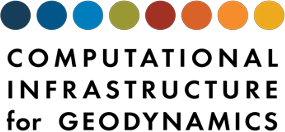
\includegraphics[scale=1.5]{../../logos/cig_logo_dots}%
  \hspace{4em}%
\raisebox{1em}{\includegraphics[scale=1.0]{../../logos/cig_short_pylith}}}
\date{June 8, 2026}


% TODO - Update mesh generator (add HDF5)

% ---------------------------------------------------- CUSTOMIZATION
\usetheme{CIG}
\input{../style}

% --------------------------------------------------------- DOCUMENT
\begin{document}

% ------------------------------------------------------------ SLIDE
\maketitle
\logo{\includegraphics[height=4.5ex]{../../logos/cig_short_pylith}}


% ========================================================== SECTION
\section{Introduction}

% ------------------------------------------------------------ SLIDE
\begin{frame}
  \frametitle{What is PyLith?}
  \summary{}

  \begin{itemize}
    \hitem{Open-source community code for crustal deformation modeling with a focus on earthquake faulting}
    \begin{itemize}
    \item Developers seek to build and maintain a robust, flexible code for a broad user base.
    \item Developers engage the community in setting priorities for code features and capabilities.
    \item Developers work with users who want to contribute code enhancements.
    \end{itemize}
    \hitem{Goal: Accessible to new users with limited experience without impeding flexibility needed by advanced users.}
    \begin{itemize}
    \item Many components have default settings that work for the most common use cases.
    \item Advanced users can assemble complex simulations by combining and adding new components.
    \end{itemize}
  \end{itemize}

\end{frame}


% ------------------------------------------------------------ SLIDE
\begin{frame}
  \frametitle{What is PyLith used for?}
  \summary{Primary use cases}

  \begin{itemize}
  \item Forward modeling of viscoelastic relaxation following earthquakes
  \item Generating static Green's functions for 3D structure (inverting for interseismic deformation or static coseismic slip)
  \item Forward modeling of quasi-static slip on faults with friction
  \item Forward modeling of dynamic (inertia) slip on faults with friction\\
  \noindent\vdots
\end{itemize}

\end{frame}


% ------------------------------------------------------------ SLIDE
\begin{frame}
  \frametitle{What is PyLith used for?}
  \summary{Typical use cases}
  
  \only<1>{\centering\remark{Typical use cases}\par}
  \only<2>{
\includegraphics[scale=0.2]{figs/typical-Bartlow-2010}}
  \only<3>{
\includegraphics[scale=0.2]{figs/typical-Diao-etal-2018}}
  \only<4>{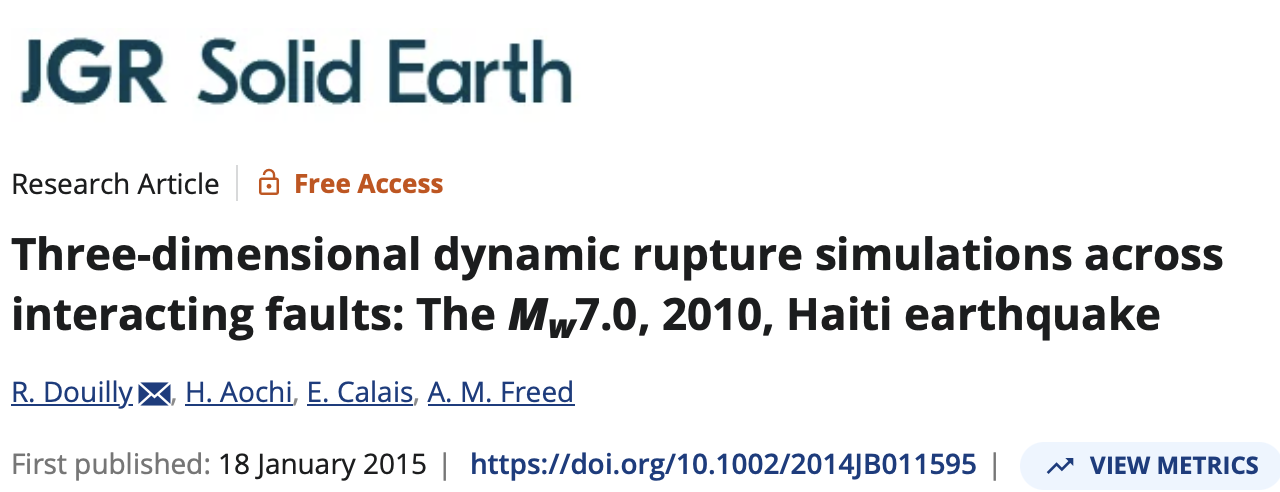
\includegraphics[scale=0.2]{figs/typical-Douilly-etal-2015}}
  \only<5>{
\includegraphics[scale=0.2]{figs/typical-Guo-etal-2020}}
  \only<6>{
\includegraphics[scale=0.2]{figs/typical-Todd-etal-2018}}
  \only<7>{
\includegraphics[scale=0.2]{figs/typical-Williams-Wallace-2018}}
  \only<8>{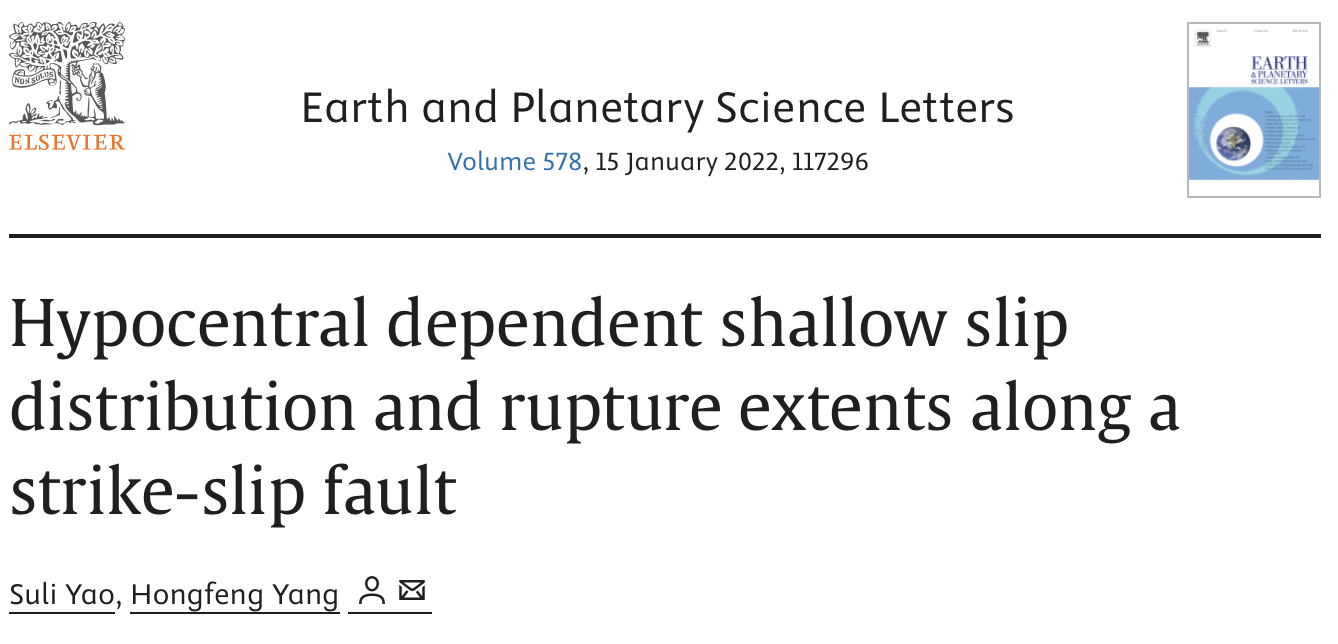
\includegraphics[scale=0.2]{figs/typical-Yao-Yang-2022}}

\end{frame}


% ------------------------------------------------------------ SLIDE
\begin{frame}
  \frametitle{What is PyLith used for?}
  \summary{Atypical use cases}

  \only<1>{\centering\remark{Atypical use cases}\par}
  \only<2>{
\includegraphics[scale=0.2]{figs/atypical-Berne-etal-2023}}
  \only<3>{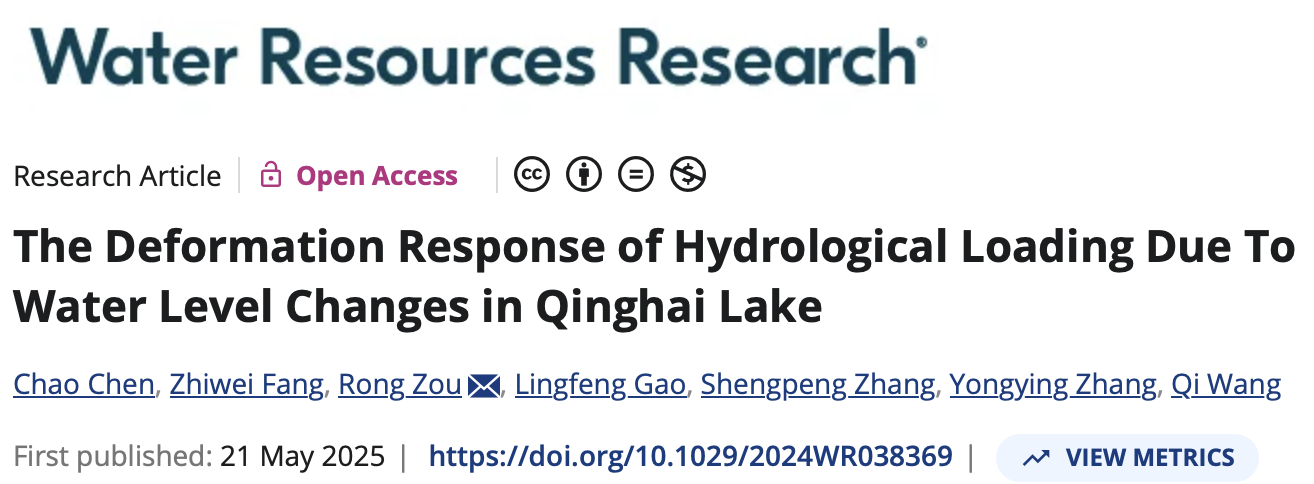
\includegraphics[scale=0.2]{figs/atypical-Chen-etal-2025}}
  \only<4>{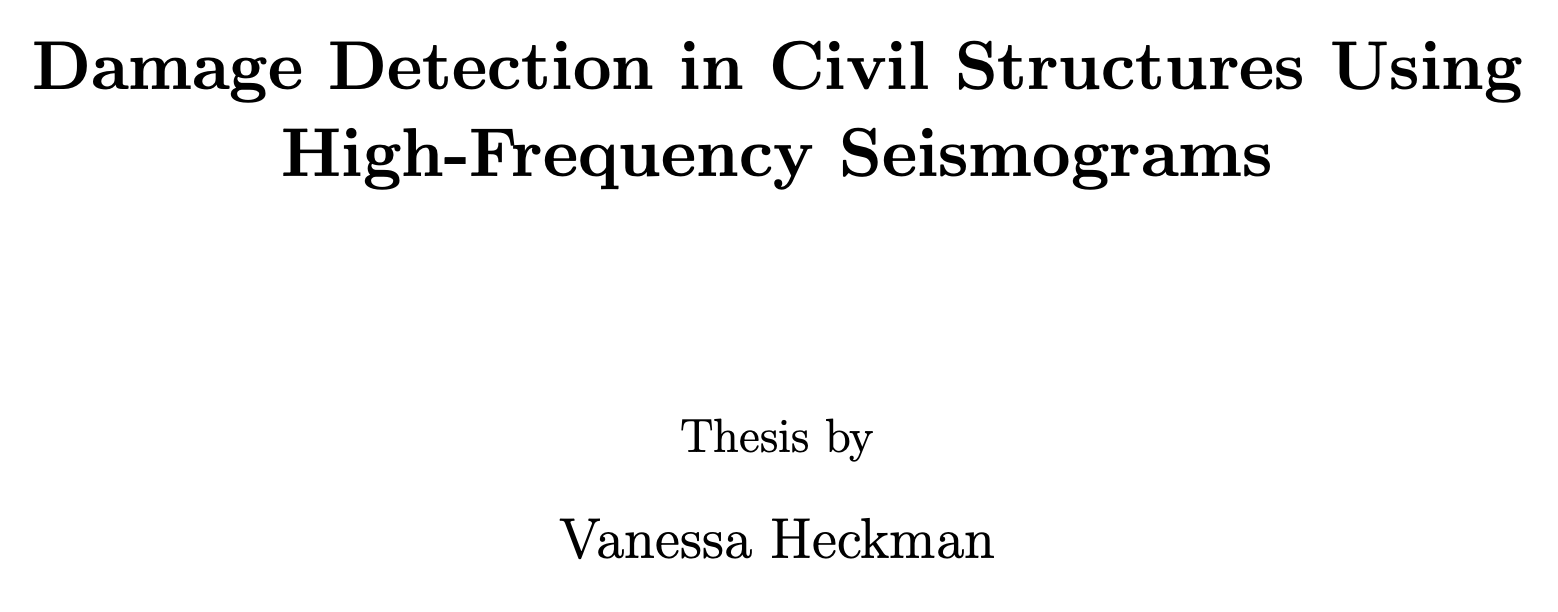
\includegraphics[scale=0.2]{figs/atypical-Heckman-2013}}
  \only<5>{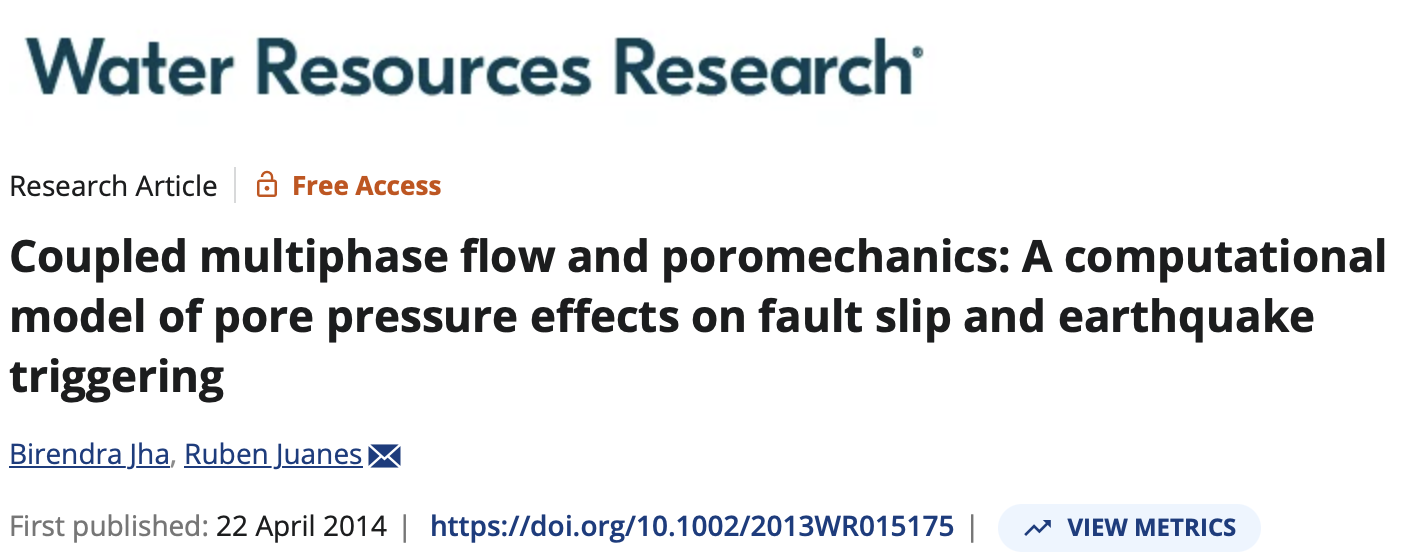
\includegraphics[scale=0.2]{figs/atypical-Jha-Juanes-2014}}
  \only<6>{
\includegraphics[scale=0.2]{figs/atypical-McLaskey-etal-2014}}
  \only<7>{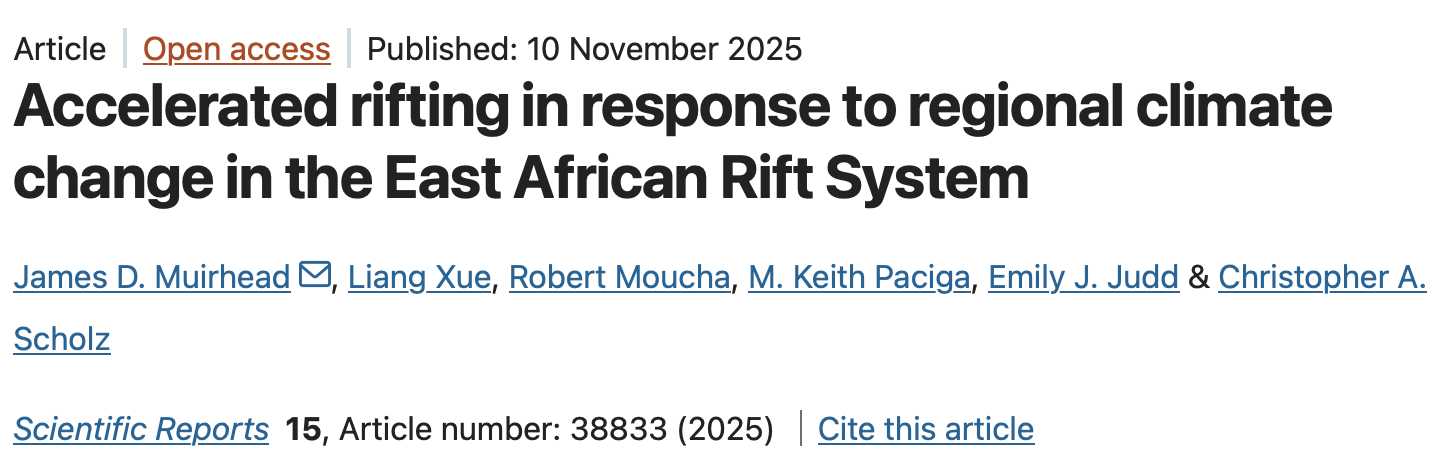
\includegraphics[scale=0.2]{figs/atypical-Muirhead-etal-2025}}
  \only<8>{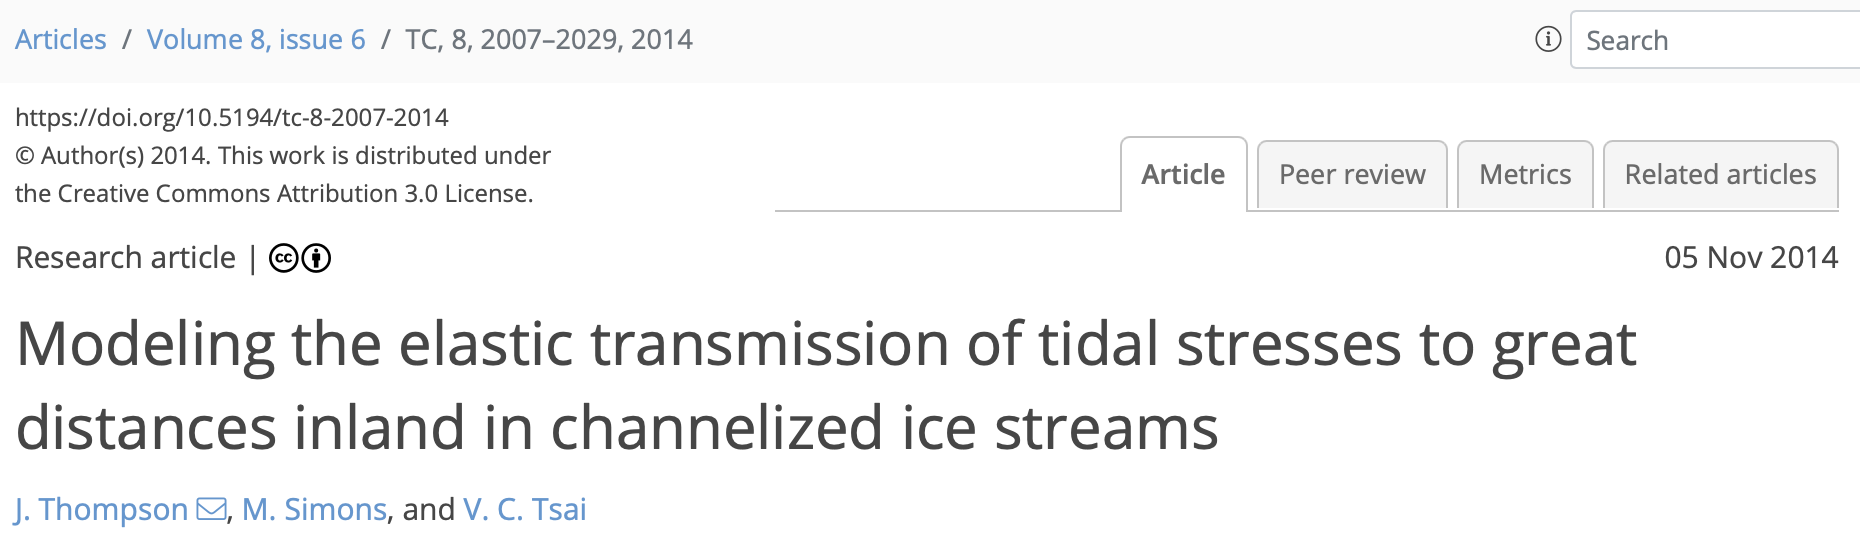
\includegraphics[scale=0.2]{figs/atypical-Thompson-etal-2014}}

\end{frame}


% ------------------------------------------------------------ SLIDE
\begin{frame}[t]
  \frametitle{Impact of PyLith}
  \summary{}

  \highlight{Our estimate is 1000--3000 studies have used PyLith since its initial release in 2007.}

  \vfill
  \begin{itemize}
  \item We do \underline{not} embed any tracking code in PyLith.
  \item We track downloads of binary distributions and source code tarballs via GitHub.
  \item We request that users self report publications that use PyLith (CIG website).
  \item We request users cite the software version (DOI $\rightarrow$ archive on Zenodo) and our publications about PyLith (mainly 2013 JGR paper).
  \end{itemize}

\end{frame}


% ------------------------------------------------------------ SLIDE
\begin{frame}[t]
  \frametitle{Quantifying the impact of PyLith}
  \summary{}

  \highlight{Our estimate is 1000--3000 studies have used PyLith since its initial release in 2007.}

  \vfill
  \remark{Nearly 400 citations of the PyLith JGR paper (Aagaard et al., 2013) since publication.}
  \begin{enumerate}
  \item Use of PyLith in research (300+ papers; 30+ papers with 50+ citations)
  \item Build on techniques, algorithms, etc. used in PyLith (12+ papers)
  \item Example of a code for specific applications, using specific techniques, or open-source code development (10+ papers)
  \end{enumerate}
  
  \vfill
  \remark{More than 10,000 downloads across 10 versions over the past 8 years.}

\end{frame}


% ------------------------------------------------------------ SLIDE
\begin{frame}
  \frametitle{Developing and Maintaining PyLith}
  \summary{It takes a sustained effort to maintain a code for nearly 20 years!}
  
  \begin{itemize}
  \hitem{Code has undergone multiple major overhauls (more planned)}
    \begin{onlyenv}<1>
      \begin{itemize}
      \item Changes in underlying data structures
      \item Changes to mathematical formulation
      \item Python 2 $\rightarrow$ Python 3
      \item CppUnit test framework $\rightarrow$ Catch2 test framework
      \end{itemize}
    \end{onlyenv}
  \hitem{Hardware has evolved}
    \begin{onlyenv}<2>    
      \begin{itemize}
      \item 32-bit operating systems
      \item Apple: PowerPC (32 bit) $\rightarrow$ x86\_64 $\rightarrow$ arm64
      \item Linux i686 (32 bit) $\rightarrow$ x86\_64
      \end{itemize}
    \end{onlyenv}    
  \hitem{Software development has changed}
    \begin{onlyenv}<3>
      \begin{itemize}
      \item CIG-hosted Subversion repository $\rightarrow$ GitHub-hosted Git repository
      \item Development on single branch $\rightarrow$ Git forking workflow
      \item CIG-hosted buildbots $\rightarrow$ Cloud-based Azure pipelines
      \item Text editors $\rightarrow$ VS Code IDE
      \end{itemize}
    \end{onlyenv}
  \hitem{User support has changed}
    \begin{onlyenv}<4>
      \begin{itemize}
      \item Build from source $\rightarrow$ binary packages
      \item \LaTeX produced PDF manual $\rightarrow$ Markdown produced online + PDF manual
      \item Mailing list $\rightarrow$ online forum
      \end{itemize}
    \end{onlyenv}
  \end{itemize}

\end{frame}


% ------------------------------------------------------------ SLIDE
\begin{frame}[t]
\frametitle{People}

{\scriptsize
\begin{tabular}{p{0.48\textwidth}p{0.48\textwidth}}
  \begin{minipage}{2.5cm}
    
\includegraphics[height=2.5cm]{figs/brad.jpg}
  \end{minipage}\hfill
  \begin{minipage}{0.3\textwidth}
     {\bf Brad Aagaard} \\ U.S. Geological Survey
  \end{minipage} &
\begin{minipage}{2.5cm}
    
\includegraphics[height=2.5cm]{figs/charles.jpg}
  \end{minipage}\hfill
  \begin{minipage}{0.3\textwidth}
     {\bf Charles Williams} \\ RPI $\rightarrow$ Earth Sciences New Zealand (formerly GNS Science)
  \end{minipage}
   \\[2cm]
\begin{minipage}{2.5cm}
    
\includegraphics[height=2.5cm]{figs/matt.jpg}
  \end{minipage}\hfill
  \begin{minipage}{0.3\textwidth}
{\bf Matt Knepley} \\ ANL $\rightarrow$ Rice $\rightarrow$ Univ. at Buffalo
  \end{minipage} &
\begin{minipage}{2.5cm}
    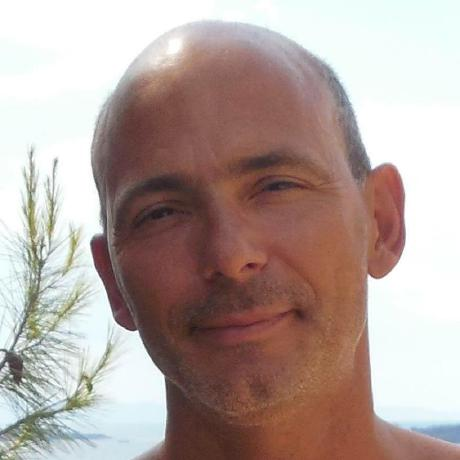
\includegraphics[height=2.5cm]{figs/michael.jpg}
  \end{minipage}\hfill
  \begin{minipage}{0.3\textwidth}
     {\bf Michael Aivazis} \\ Caltech CACR $\rightarrow$ ? $\rightarrow$ ParaSim
  \end{minipage}
      \\
\end{tabular}}

\end{frame}

% ------------------------------------------------------------ SLIDE
\begin{frame}
\frametitle{Contributors to upcoming and recent releases}

Grant Block 
\includegraphics[height=1em]{images/ORCIDiD_icon32x32}0009-0003-3402-0923 \\
Daniel Douglas 
\includegraphics[height=1em]{images/ORCIDiD_icon32x32}0000-0002-7871-018X \\
Lorraine Hwang 
\includegraphics[height=1em]{images/ORCIDiD_icon32x32}0000-0002-1021-3101 \\
Evan Marschall 
\includegraphics[height=1em]{images/ORCIDiD_icon32x32}0009-0003-0916-6656 \\
Ritwik Patil 
\includegraphics[height=1em]{images/ORCIDiD_icon32x32}0009-0008-3305-6728 \\
Rezgar Shakeri 
\includegraphics[height=1em]{images/ORCIDiD_icon32x32}0000-0003-4790-7016 \\
Robert Walker 
\includegraphics[height=1em]{images/ORCIDiD_icon32x32}0000-0001-7856-1949 \\
Peng Zhai 
\includegraphics[height=1em]{images/ORCIDiD_icon32x32}0000-0001-5899-4421 \\
Zechao Zhuo 
\includegraphics[height=1em]{images/ORCIDiD_icon32x32}0000-0002-8163-5731

\end{frame}

% ------------------------------------------------------------ SLIDE
\begin{frame}[t]
  \frametitle{A brief history of PyLith}

  \begin{overlayarea}{\textwidth}{7.1cm}
    \only<1>{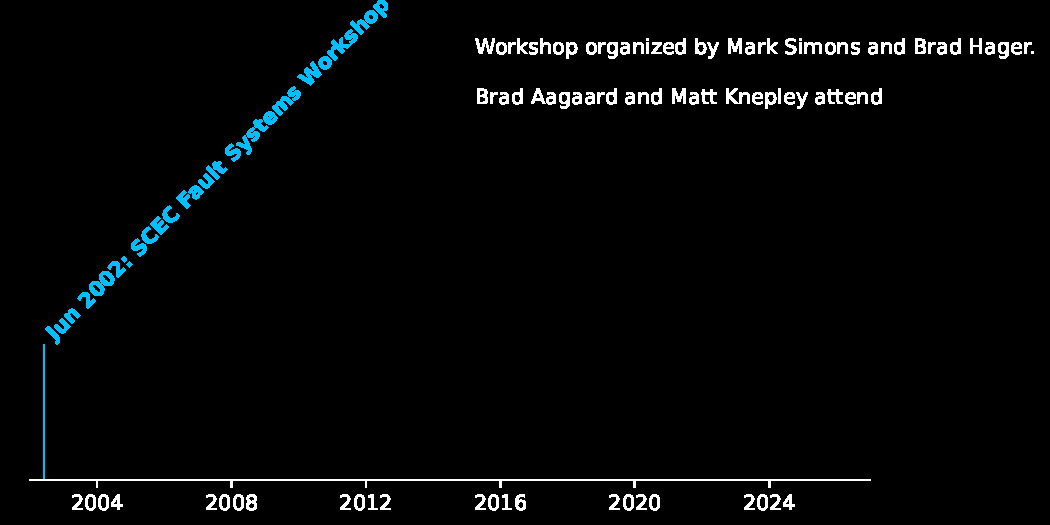
\includegraphics[height=6.9cm]{figs/pylith-timeline-00}}
    \only<2>{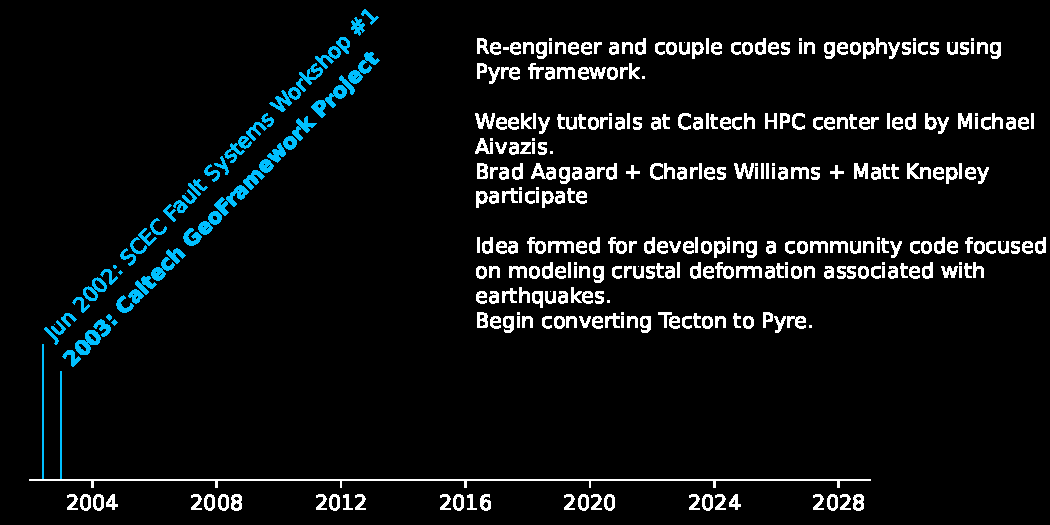
\includegraphics[height=6.9cm]{figs/pylith-timeline-01}}
    \only<3>{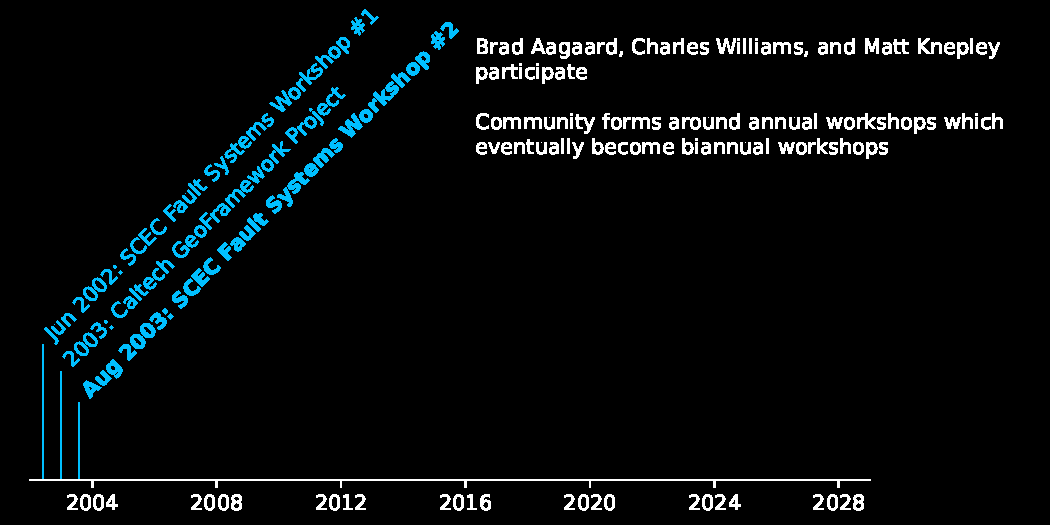
\includegraphics[height=6.9cm]{figs/pylith-timeline-02}}
    \only<4>{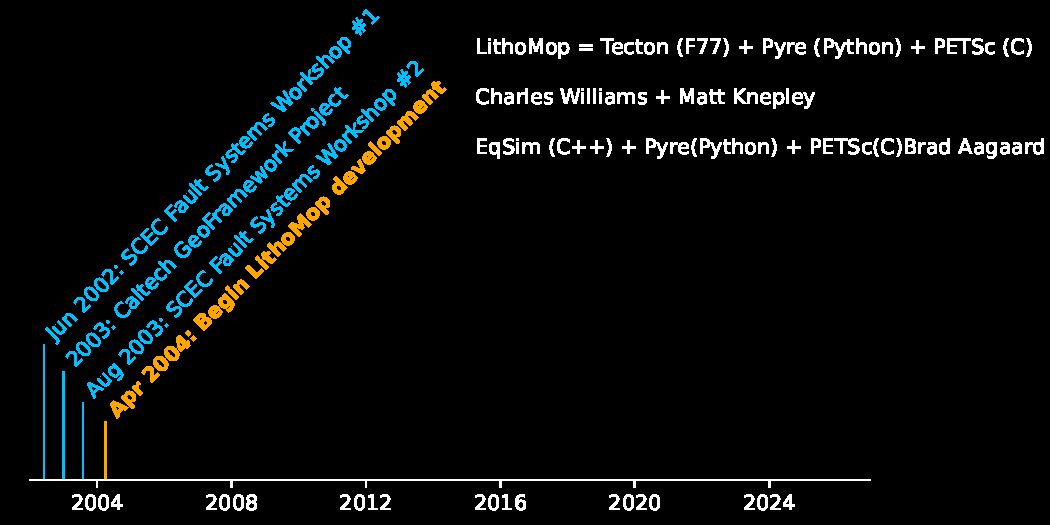
\includegraphics[height=6.9cm]{figs/pylith-timeline-03}}
    \only<5>{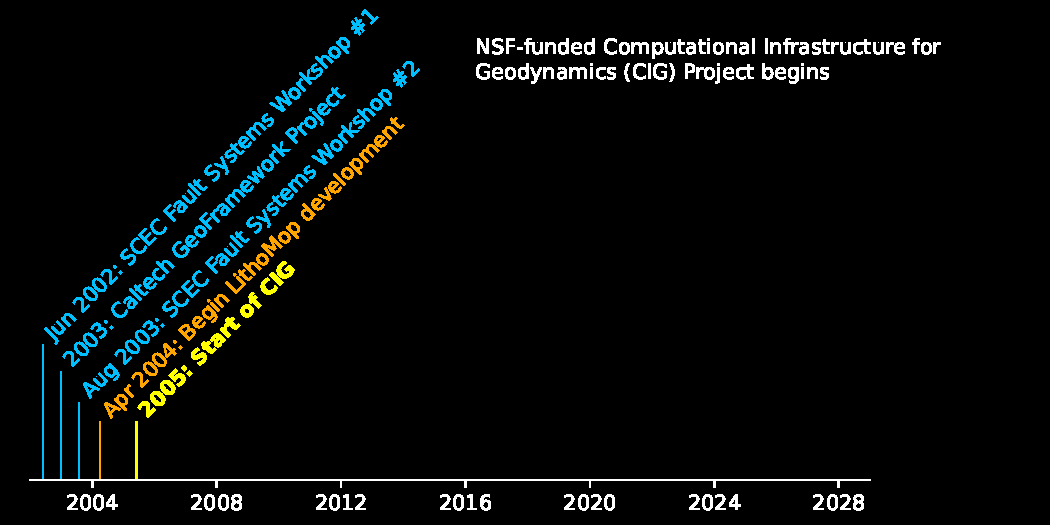
\includegraphics[height=6.9cm]{figs/pylith-timeline-04}}
    \only<6>{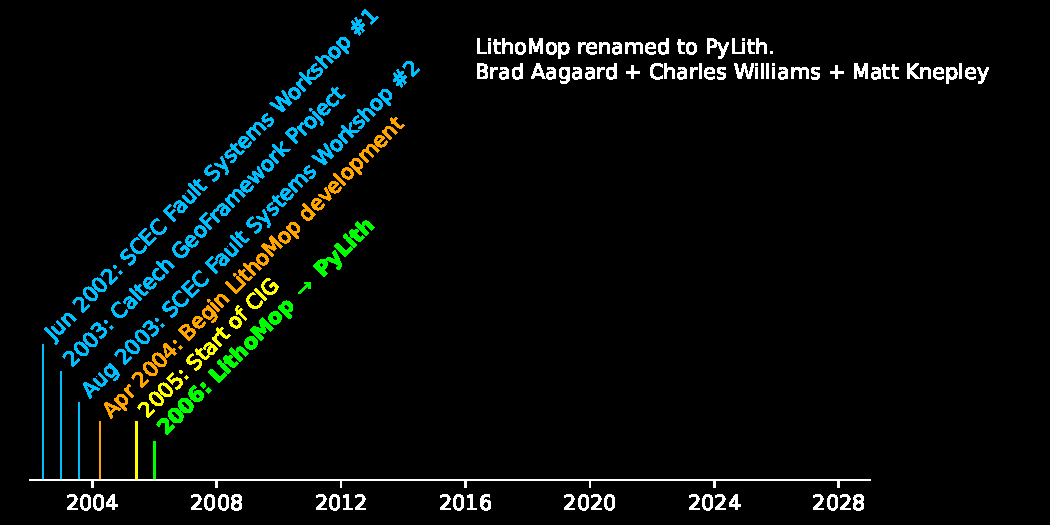
\includegraphics[height=6.9cm]{figs/pylith-timeline-05}}
    \only<7>{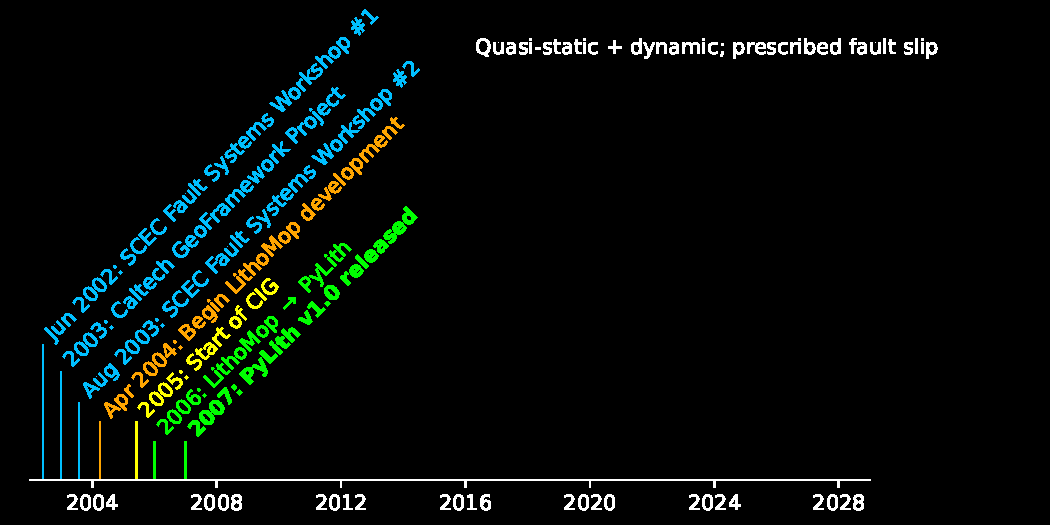
\includegraphics[height=6.9cm]{figs/pylith-timeline-06}}
    \only<8>{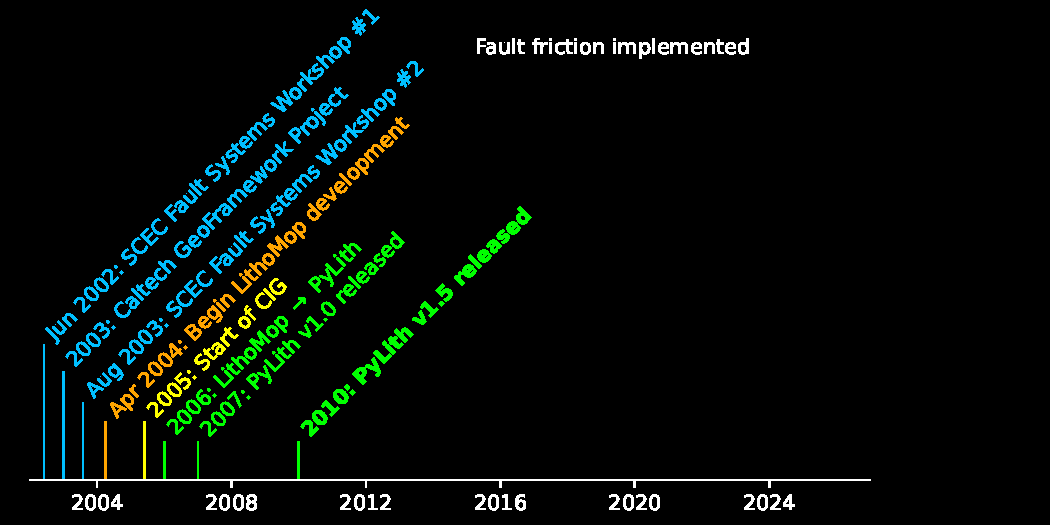
\includegraphics[height=6.9cm]{figs/pylith-timeline-07}}
    \only<9>{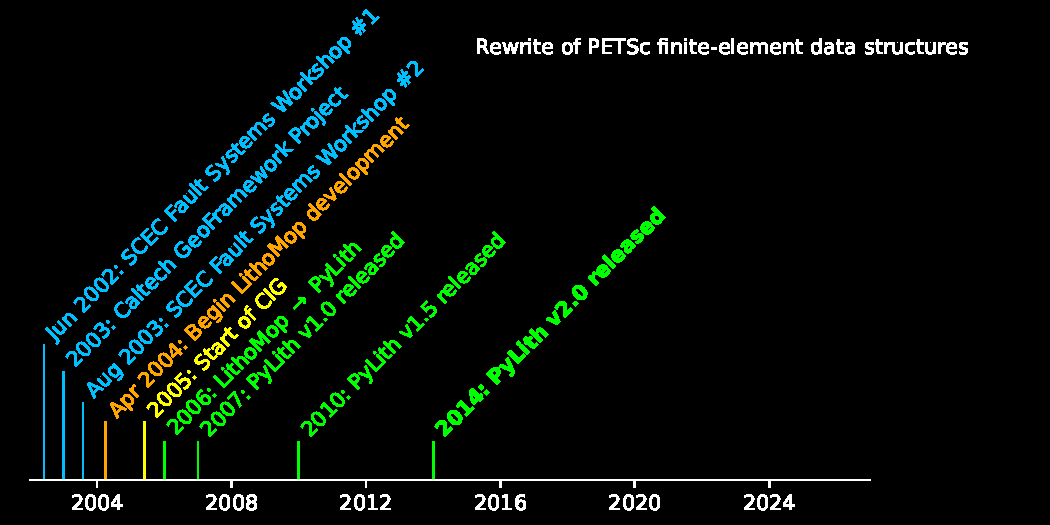
\includegraphics[height=6.9cm]{figs/pylith-timeline-08}}
    \only<10>{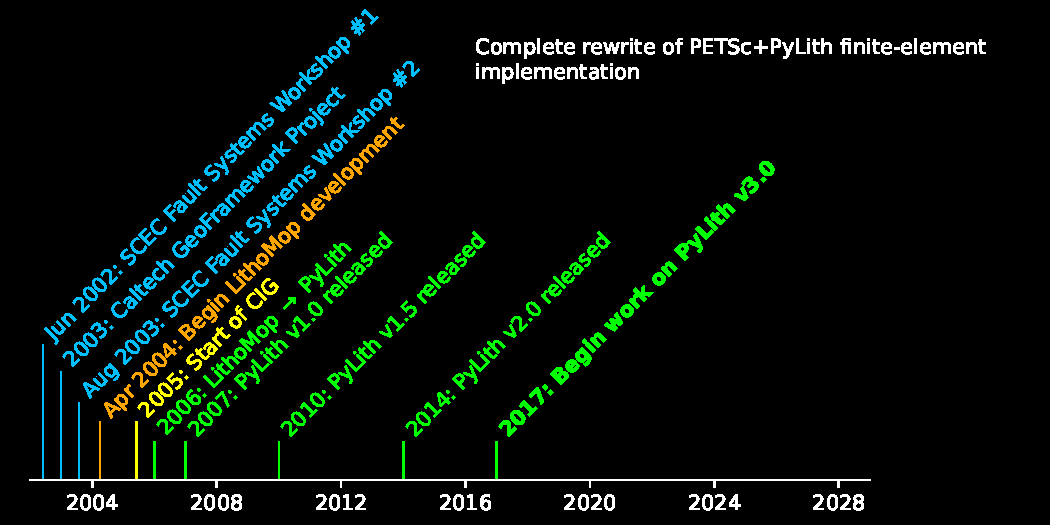
\includegraphics[height=6.9cm]{figs/pylith-timeline-09}}
    \only<11>{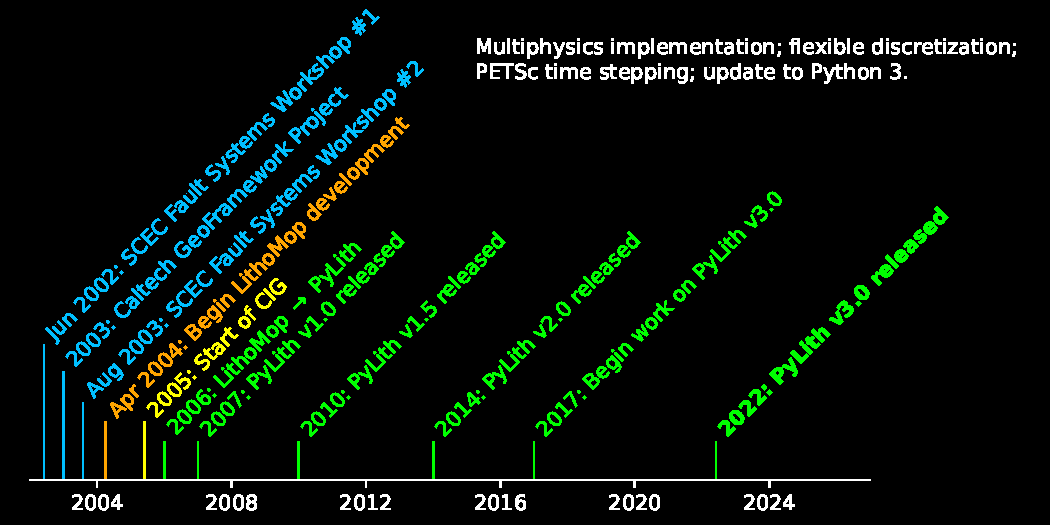
\includegraphics[height=6.9cm]{figs/pylith-timeline-10}}
    \only<12>{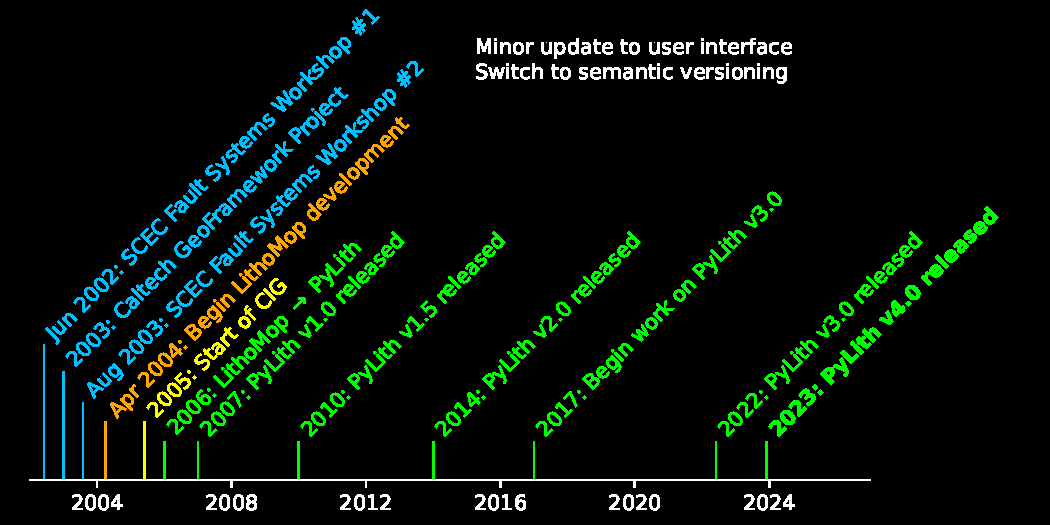
\includegraphics[height=6.9cm]{figs/pylith-timeline-11}}
    \only<13>{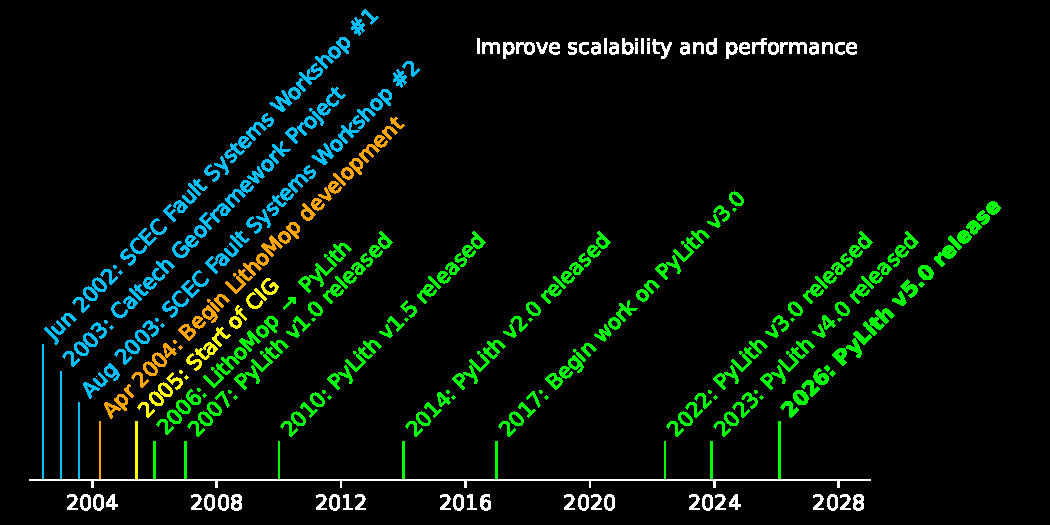
\includegraphics[height=6.9cm]{figs/pylith-timeline-12}}
    \only<13>{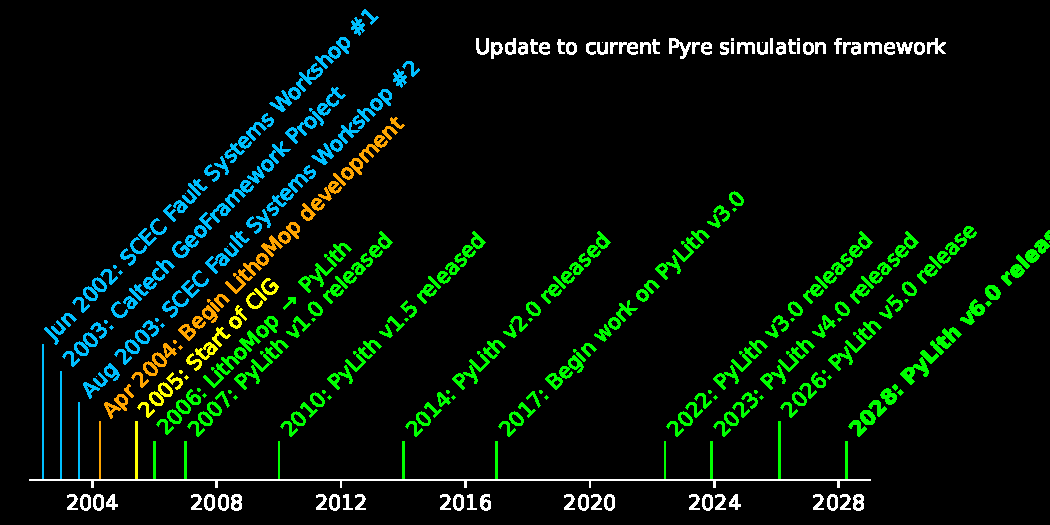
\includegraphics[height=6.9cm]{figs/pylith-timeline-13}}
  \end{overlayarea}

\end{frame}


% ========================================================== SECTION
\section{PyLith v5.0}

% ------------------------------------------------------------ SLIDE
\begin{frame}
  \frametitle{PyLith v3}
  \summary{Major rewrite of PyLith, 2016--2022}

  \footnotesize{\begin{tabular}{p{3.0cm}p{5.0cm}p{5.0cm}}
    \toprule
    Feature
    & PyLith v2
    & PyLith v3 \\
    \midrule
    Governing eqn
    & Hardwired (elasticity)
    & Flexible (elasticity, incompressible elasticity, poroelasticity)
    \\[2em]
    Temporal discretization
    & Backward Euler, Newmark (central difference)
    & PETSc TS (primarily Runge Kutta)
      \\[2em]
    Spatial discretization
    & Hardwired (1st order)
    & Flexible (tested up to 4th order)
           \\[1em]
           Finite-element definition
           & PyLith
           & PETSc \\
    \bottomrule
  \end{tabular}}
    
\end{frame}


% ------------------------------------------------------------ SLIDE
\begin{frame}
  \frametitle{PyLith v4.2 $\rightarrow$ PyLith v5.0}
  \summary{}

  \begin{itemize}
  \item v5.0 is very similar to v4.x; a few small changes to parameter files
  \item v5.0 includes scalable mesh loading and processing, updates to the 3D subduction zone example, improved performance, and bugfixes
  \end{itemize}

  \vfill\pause

  Starting with PyLith v3.0.0 we follow semantic versioning guidelines more closely.\\
  Version numbers convey impact on user, not necessarily amount of change to the code.

  \begin{description}
  \item[Major release] Changes to user interface (breaks backward compatibility)
  \item[Minor release] New features and bugfixes (backward compatible)
  \item[Patch release] Bug fixes
  \end{description}
    
\end{frame}


% ------------------------------------------------------------ SLIDE
\begin{frame}
  \frametitle{PyLith v5.0}
  \summary{}

  \begin{itemize}
  \item Most features from v2.2 have been reimplemented, tested, and documented
  \item A few additional features and under-the-hood improvements are almost ready
    \begin{itemize}
    \item Elasticity with inertia and prescribed fault slip
    \end{itemize}
  \item A few major features in v2.2 have not yet been implemented
    \begin{itemize}
    \item Spontaneous fault rupture (fault friction)
    \item Small strain formulation for elasticity
    \end{itemize}    
  \end{itemize}

\end{frame}

\newcommand{\statuslater}[1]{{\color{purple}#1}}
\newcommand{\statusdone}[1]{{\color{green}#1}}
\newcommand{\statusbuggy}[1]{{\color{red}#1}}
\newcommand{\statusinprogress}[1]{{\color{orange}#1}}
% ------------------------------------------------------------ SLIDE
\begin{frame}
  \frametitle{PyLith v5.0: Governing Equations}
  \summary{}

  Elasticity
  \begin{itemize}
  \item \statusdone{Static and quasi-static problems}
  \item \statusinprogress{Dynamic problems (with inertia)}
  \item \statusdone{Infinitesimal strains}
  \item \statusinprogress{Small strain}
  \item \statusdone{Gravitational body forces}
  \item \statusdone{Body forces}
  \item Bulk rheologies (constitutive models)
    \begin{itemize}
    \item \statusdone{Isotropic, linear elasticity}
    \item \statusdone{Isotropic, linear Maxwell viscoelasticity}
    \item \statusdone{Isotropic, linear generalized Maxwell viscoelasticity}
    \item \statusdone{Isotropic, power-law viscoelasticity}
    \item \statusinprogress{Isotropic, Drucker-Prager elastoplasticity}
    \end{itemize}
  \end{itemize}
  \vfill\hfill%
  \begin{minipage}{0.25\textwidth}
    \statusdone{Done}\\
    %\statusbuggy{Buggy}\\
    \statusinprogress{In Progress}\\
    \statuslater{Coming Later}
  \end{minipage}  
\end{frame}

% ------------------------------------------------------------ SLIDE
\begin{frame}
  \frametitle{PyLith v5.0: Governing Equations}
  \summary{}

  Poroelasticity
  \begin{itemize}
  \item \statusdone{Static and quasi-static problems}
  \item \statusdone{Infinitesimal strains}
  \item \statusdone{Gravitational body forces}
  \item \statusdone{Body forces}
  \item Bulk rheologies (constitutive models)
    \begin{itemize}
    \item \statusdone{Isotropic, linear elasticity}
    \item \statusinprogress{Isotropic, linear viscoelasticity}
    \end{itemize}
  \item \statusdone{Prescribed slip without poroelastic coupling across fault}
  \item \statusinprogress{Prescribed slip with poroelastic fault properties}
  \end{itemize}
  \vfill\hfill%
  \begin{minipage}{0.25\textwidth}
    \statusdone{Done}\\
    %\statusbuggy{Buggy}\\
    \statusinprogress{In Progress}\\
    \statuslater{Coming Later}
  \end{minipage}  

\end{frame}


% ------------------------------------------------------------ SLIDE
\begin{frame}
  \frametitle{PyLith v5.0: Governing Equations}
  \summary{}

  Incompressible elasticity
  \begin{itemize}
  \item \statusdone{Static and quasi-static problems}
  \item \statusdone{Infinitesimal strains}
  \item \statusdone{Gravitational body forces}
  \item \statusdone{Body forces}
  \item Bulk rheologies (constitutive models)
    \begin{itemize}
    \item \statusdone{Isotropic, linear elasticity}
    \end{itemize}
  \end{itemize}

  \vfill\hfill%
  \begin{minipage}{0.25\textwidth}
    \statusdone{Done}\\
    %\statusbuggy{Buggy}\\
    \statusinprogress{In Progress}\\
    \statuslater{Coming Later}
  \end{minipage}  

\end{frame}


% ------------------------------------------------------------ SLIDE
\begin{frame}
  \frametitle{PyLith v5.0: Boundary and Interface Conditions}
  \summary{}

  \begin{itemize}
  \item Boundary conditions
    \begin{itemize}
    \item \statusdone{Simple time-dependent Dirichlet boundary conditions}
    \item \statusdone{Simple time-dependent Neumann (traction) boundary conditions}
    \item \statusdone{Absorbing boundary conditions}
    \item \statuslater{Boundary conditions with complex spatial and temporal variations}
    \end{itemize}
  \item Interface conditions
    \begin{itemize}
    \item \statusdone{Kinematic (prescribed slip) fault interfaces w/multiple ruptures}
    \item \statusinprogress{Dynamic (friction) fault interfaces}
      \begin{itemize}
      \item \statusinprogress{Static friction}
      \item \statuslater{Linear slip-weakening}
      \item \statuslater{Linear time-weakening}
      \item \statuslater{Dieterich-Ruina rate and state friction w/aging law}
      \end{itemize}
    \end{itemize}
  \end{itemize}
  \hfill%
  \begin{minipage}{0.25\textwidth}
    \statusdone{Done}\\
    %\statusbuggy{Buggy}\\
    \statusinprogress{In Progress}\\
    \statuslater{Coming Later}
  \end{minipage}  

\end{frame}


% ------------------------------------------------------------ SLIDE
\begin{frame}
  \frametitle{PyLith v5.0: Other Features}
  \summary{}

  \begin{itemize}
  \item Importing meshes
    \begin{itemize}
    \item \statusdone{Gmsh}
    \item \statusdone{Cubit: Exodus II}
    \item \statusdone{ASCII: PyLith mesh ASCII format (intended for toy problems only)}
    \item \statusdone{PETSc HDF5: parallel mesh loading}
    \end{itemize}
  \item \statusdone{Initial conditions}
  \item Output: HDF5 and VTU files
    \begin{itemize}
    \item \statusdone{Solution over domain}
    \item \statusdone{Solution over domain boundary}
    \item \statusdone{Solution interpolated to user-specified points w/station
      names}
    \item \statusdone{Solution over materials and boundary conditions}
    \item \statusdone{State variables (e.g., stress and strain) for each material}
    \item \statusdone{Fault information (e.g., slip and tractions)}
    \end{itemize}
 \end{itemize}
  \hfill%
  \begin{minipage}{0.25\textwidth}
    \statusdone{Done}\\
    %\statusbuggy{Buggy}\\
    \statusinprogress{In Progress}\\
    \statuslater{Coming Later}
  \end{minipage}  
  
\end{frame}


% ------------------------------------------------------------ SLIDE
\begin{frame}
  \frametitle{PyLith v5.0: Other Features  (cont.)}
  \summary{}

  \begin{itemize}
  \item \statusdone{Automatic conversion of units for all parameters}
  \item \statusdone{Parallel uniform global refinement}
  \item \statusdone{PETSc linear and nonlinear solvers}
  \item \statusdone{Output of simulation progress estimates runtime}
  \item \statusdone{Default PETSc options based on material (governing equation)}
 \end{itemize}
  \vfill\hfill%
  \begin{minipage}{0.25\textwidth}
    \statusdone{Done}\\
    %\statusbuggy{Buggy}\\
    \statusinprogress{In Progress}\\
    \statuslater{Coming Later}
  \end{minipage}  
  
\end{frame}


% ========================================================== SECTION
\section{Finite-Element Formulation}

\abovedisplayskip=2pt
\abovedisplayshortskip=2pt
\belowdisplayskip=2pt
\belowdisplayshortskip=2pt

% ------------------------------------------------------------ SLIDE
\begin{frame}
  \frametitle{Governing Equations}
  \summary{}

  \begin{itemize}
  \item Elasticity
  \item Incompressible elasticity
  \item Poroelasticity
  \end{itemize}

  \vfill
  \highlight{Refer to the Governing Equations section of the PyLith manual for more detail}
  
  
\end{frame}

% ------------------------------------------------------------ SLIDE
\begin{frame}
  \frametitle{Aside: Finite-Element Method}
  \summary{Discretization}

  \begin{itemize}
  \item Divide a domain into ``cells'' (triangles, quadrilaterals, tetrahedra, hexahedra)
  \item Represent a ``field'' within each cell using ``basis'' functions
    \begin{itemize}
    \item Often use polynomials, but we can use other types of functions too
    \item Refer to finite-element textbooks for details about functional forms of basis functions
      \begin{onlyenv}<2>
    \item Basis functions in 1D
      \begin{description}
      \item[basis order 0] $\phi(x) = a_0$
      \item[basis order 1] $\phi(x) = a_0 + a_1 x$
      \item[basis order 2] $\phi(x) = a_0 + a_1 x + a_2 x^2$
      \end{description}
    \end{onlyenv}
    \begin{onlyenv}<3>
  \item Basis functions in 2D
      \begin{description}
      \item[basis order 0] $\phi(x, y) = a_0$
      \item[basis order 1] $\phi(x, y) = a_0 + a_1 x + b_1 y$
      \item[basis order 2] $\phi(x, y) = a_0 + a_1 x + b_1 y + a_2 x^2 + b_2 y^2 + c_2 x y$
      \end{description}
    \end{onlyenv}
  \end{itemize}
  \item Compute integral as a sum of evaluations of functionals at points
    \begin{itemize}
    \item Choose point locations to minimize errors in integrals for given basis functions
    \item $F(x,y) = \sum_\mathit{cells} w_i f(\phi(x_i))$
    \end{itemize}
  \end{itemize}

\end{frame}

  
% ------------------------------------------------------------ SLIDE
\begin{frame}
  \frametitle{Formulation of governing equations}
  \summary{}

  \href{run:movies/formulation.mp4}{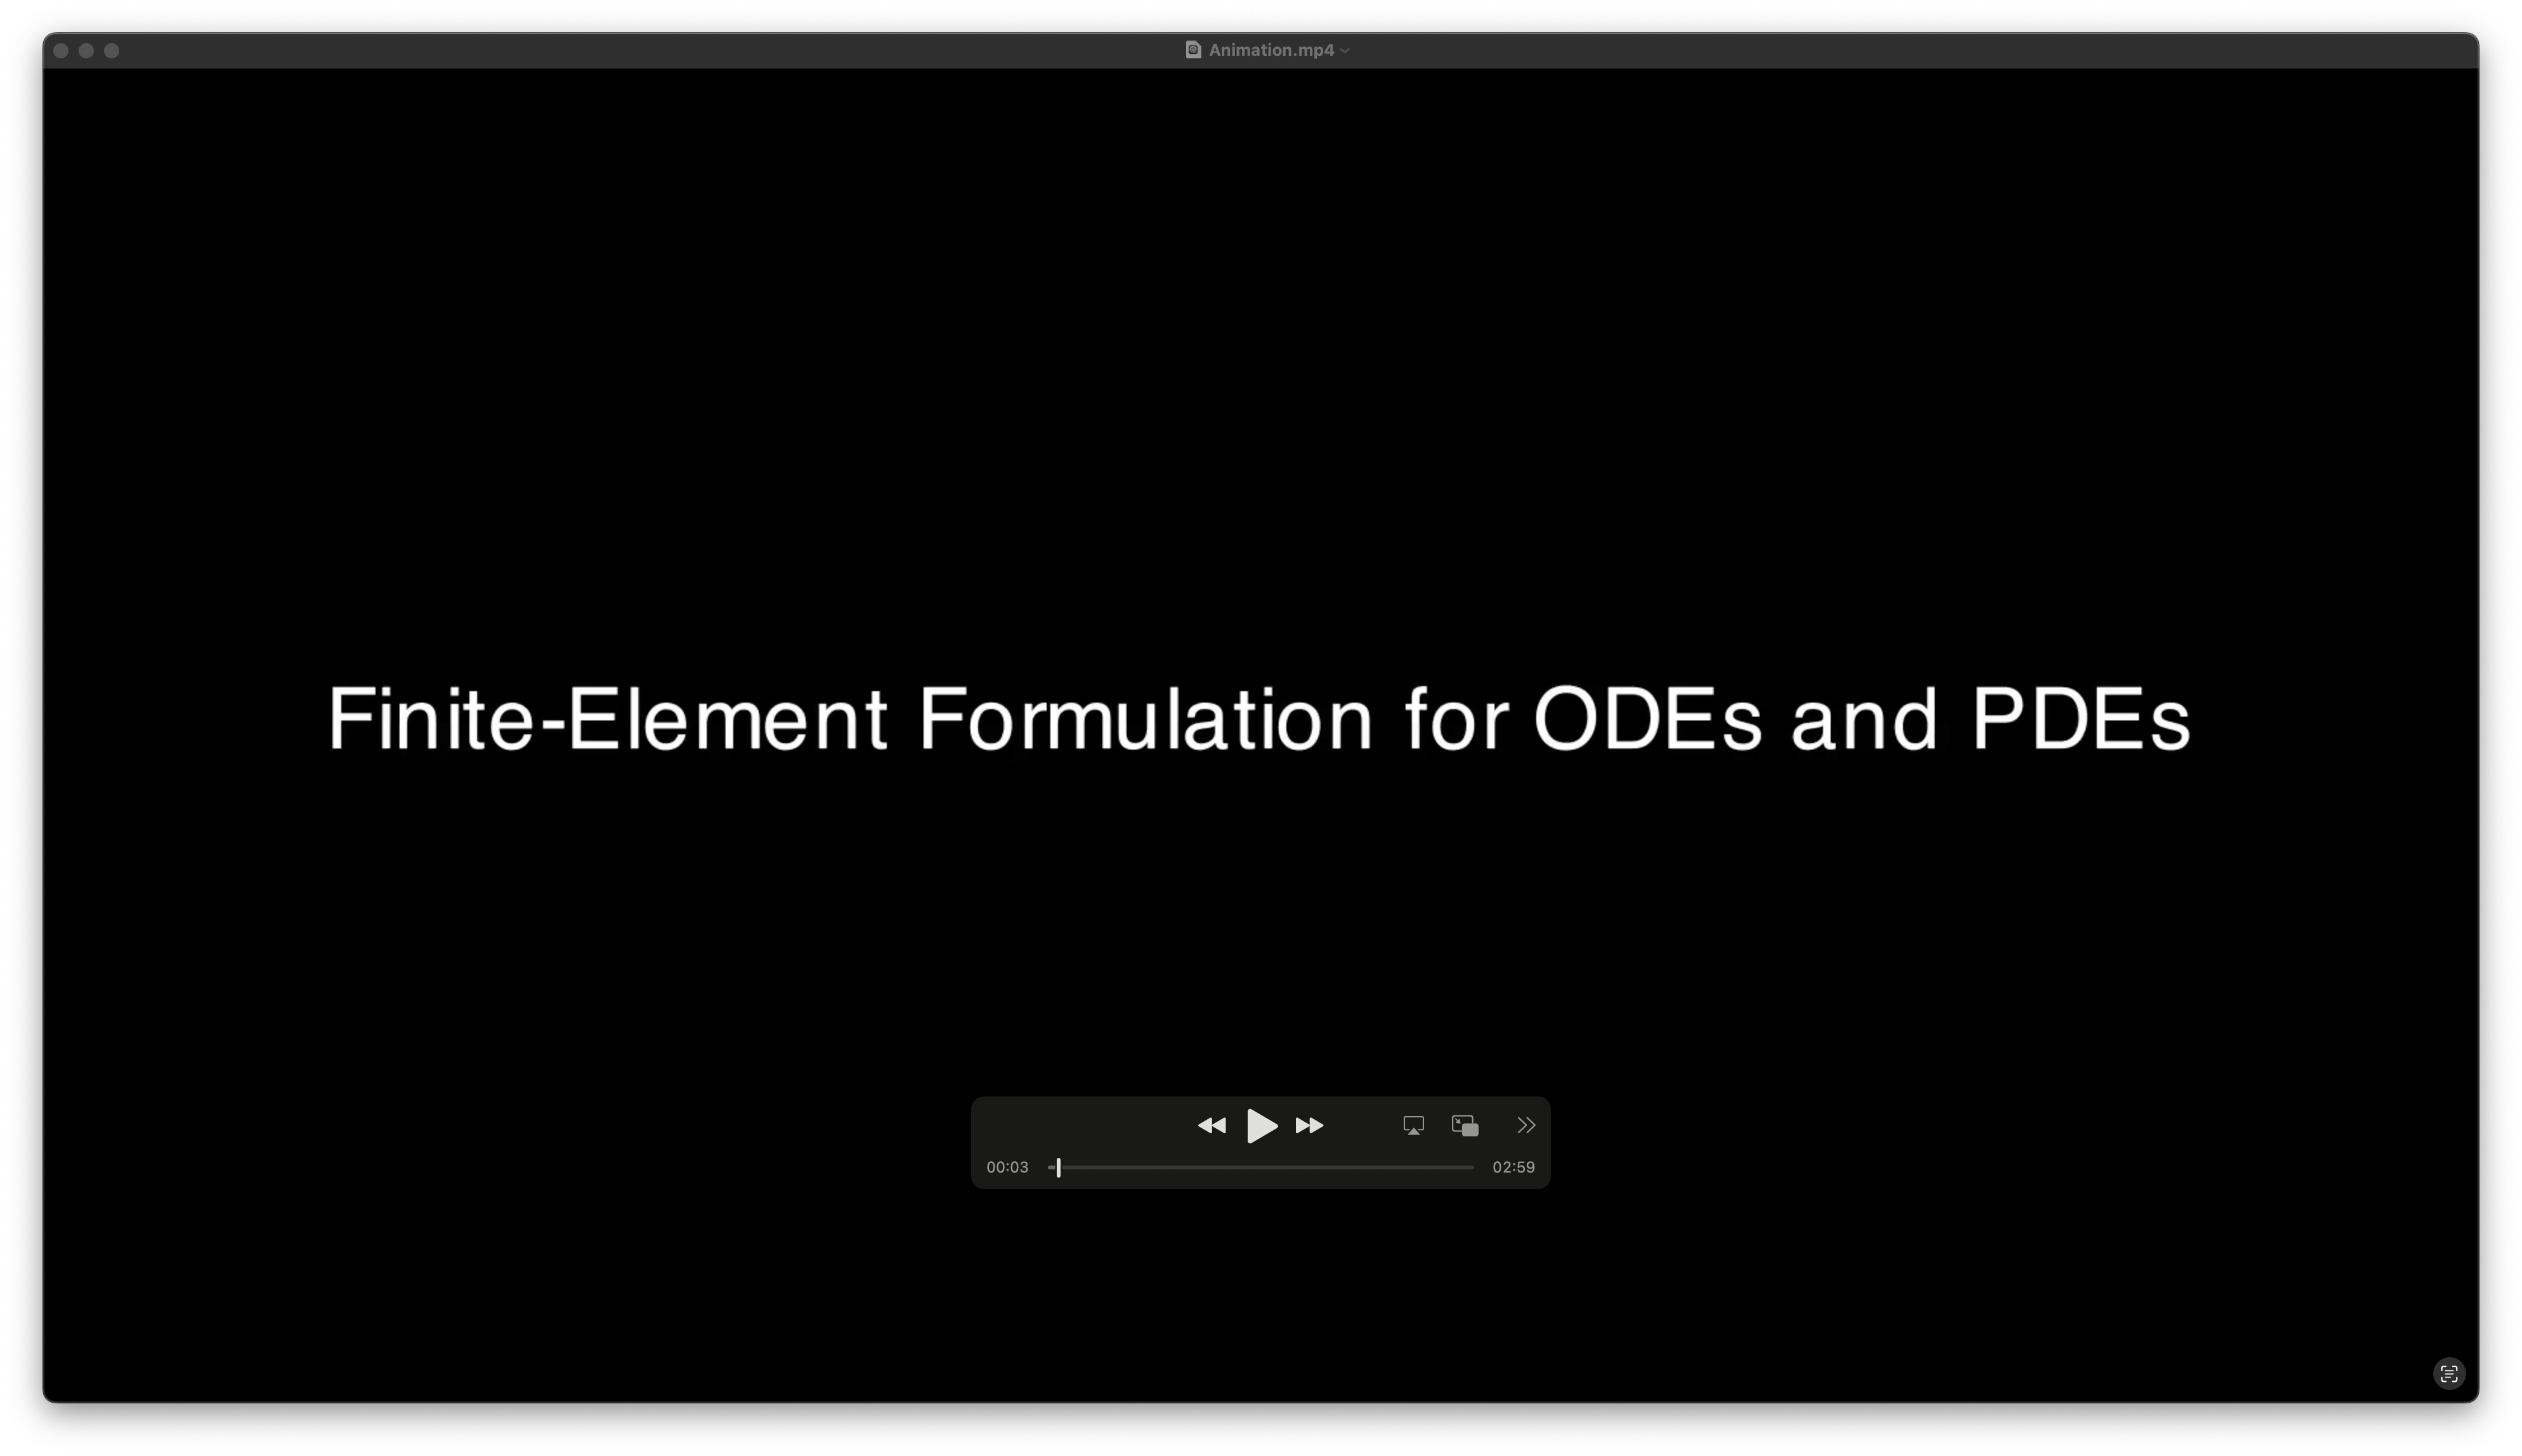
\includegraphics[width=\textwidth]{movies/formulation}}
  
\end{frame}


% ------------------------------------------------------------ SLIDE
\begin{frame}[t]
  \frametitle{Nondimensionalization}
  \summary{}

\begin{equation}
\rho(\vec{x})\frac{\partial^{2}\vec{u}}{\partial t^{2}}-\vec{f}(\vec{x},t)-\boldsymbol{\nabla}\cdot\boldsymbol{\sigma}=\vec{0}\text{ in }\Omega
\end{equation}

\begin{equation}
\vec{x}^* = \frac{\vec{x}}{x_o} \quad
\vec{u}^* = \frac{\vec{u}}{u_o} \quad
\rho^* = \frac{\rho}{\rho_o} \quad
\vec{f}^* = \frac{\vec{f}}{f_o} \quad
\boldsymbol{\sigma}^* = \frac{\boldsymbol{\sigma}}{\sigma_o} \quad
\vec{\tau}^* = \frac{\vec{\tau}}{\sigma_o}
\end{equation}

\begin{equation}
\rho_o  \rho^*(\vec{x}^*) \frac{u_o}{t_o^2} \frac{\partial^{2}\vec{u}^*}{\partial {t^*}^{2}} - f_o \vec{f}^*(\vec{x}^*,t^*) - \frac{\sigma_o}{x_o} \boldsymbol{\nabla}^*\cdot\boldsymbol{\sigma}^* = \vec{0}\text{ in }\Omega
\end{equation}

\vfill
\begin{tabular}{llll}
$x_o$       & Length scale        & $\sigma_o = \mu_o \frac{u_o}{x_o}$ & Stress scale \\
$u_o$       & Displacement scale  & $f_o = \frac{\sigma_o}{x_o}$ & Body force scale \\
$\mu_o$     & Rigidity scale      & $\rho_o = \mu_o \frac{t_o^2}{x_o^2}$ & Density scale \\
$t_o$       & Time scale          & & \\
\end{tabular}

\end{frame}


% ------------------------------------------------------------ SLIDE
\begin{frame}[t]
  \frametitle{Solver for quasi-static boundary value problems}
  \summary{}

  Solve $A s = b$ in which $A$ may be nonsymmetric due to bulk rheologies.

  \vfill
  Use the Generaralized Minimal Residual (GMRES) method with restart ($A$ can be any square, invertible matrix) with the Krylov subspace iterative method.

  \vfill
  A Krylov solver builds a small model of a linear operator $A$, using a subspace defined by successive applications of $A$ to an initial residual vector:
  \begin{equation}
    \kappa(r, A) = \text{span}\{r, Ar, A^{2}r, \ldots, A^k r\}.
  \end{equation}\vspace*{-2em}
  \begin{itemize}
    \item Scalability suffers after many iterations; the solver does a lot of inner products.
    \item GMRES+KSP requires a preconditioner to be effective.
  \end{itemize}
  
\end{frame}


% ------------------------------------------------------------ SLIDE
\begin{frame}[t]
  \frametitle{Preconditioners}
  \summary{}

  Instead of solving $A s = b$ directly, solve an equivalent system:
  \begin{equation}
    P^{-1} A s = P^{-1} b,
  \end{equation}
  where $P$ is the preconditioner.

  \vfill
  A good preconditioner
  \begin{itemize}
  \item approximates $A^{-1}$, making $P^{-1}A$ close to the identity matrix, and
  \item is inexpensive to compute and apply.
  \end{itemize}
  
\end{frame}


% ------------------------------------------------------------ SLIDE
\begin{frame}
  \frametitle{Finite-Element Implementation User Interface}
  \summary{}

  \begin{itemize}
    \hitem{Pointwise functions for the residuals and Jacobian are selected automatically}\pause
    \hitem{Fields and Subfields}
    \begin{itemize}
    \item Finite-element coefficients for the basis functions (values at vertices, on edges and faces, or in cells) are stored in a \pylith{Field}
    \item A \pylith{Field} is composed of a \pylith{Section}, which associates the points (vertices, edges, faces, and cells) with the finite-element coefficients, and a PETSc \pylith{Vec}, which is a vector storing the finite-element coefficients
    \item A \pylith{Field} may hold one or more subfields, such as the density, shear modulus, and bulk modulus for an isotropic, linear elastic material
    \end{itemize}\pause
    \hitem{Discretization}
    \begin{itemize}
    \item Each subfield within a \pylith{Field} can have a different discretization (basis order)
    \item The default basis order is 1
    \item For uniform fields (uniform material properties), we use a basis order of 0 to reduce storage requirements
    \end{itemize}
  \end{itemize}

\end{frame}

% ------------------------------------------------------------ SLIDE
\begin{frame}
  \frametitle{Solution and Auxiliary Fields}
  \summary{}

  \begin{itemize}
    \hitem{Solution field}
    \begin{itemize}
    \item Subfields match the unknowns in the governing equation
    \item Contains all finite-element coefficients corresponding to the problem solution
    \item Any subfield can be output over the domain, an external boundary, or specified locations in the domain
    \end{itemize}\pause
    \hitem{Auxiliary field}
    \begin{itemize}
    \item Spatially variable parameters for materials, boundary conditions, and fault interfaces
    \item Each parameter (scalar, vector, tensor, or other) is held in a separate subfield
    \item Also holds state variables
    \item Any subfield can be output after initialization (diagnostic) or after solving the equations
    \end{itemize}
  \end{itemize}

\end{frame}


% ------------------------------------------------------------ SLIDE
\begin{frame}[fragile]
  \frametitle{Fault Interface}
  \summary{Fault tractions couple deformation across interface}

  \includefigure[height=7.0cm]{figs/domain-decomposition}

\end{frame}


% ------------------------------------------------------------ SLIDE
\begin{frame}
  \frametitle{Implementation of faults}
  \summary{}

  \href{run:movies/fault.mp4}{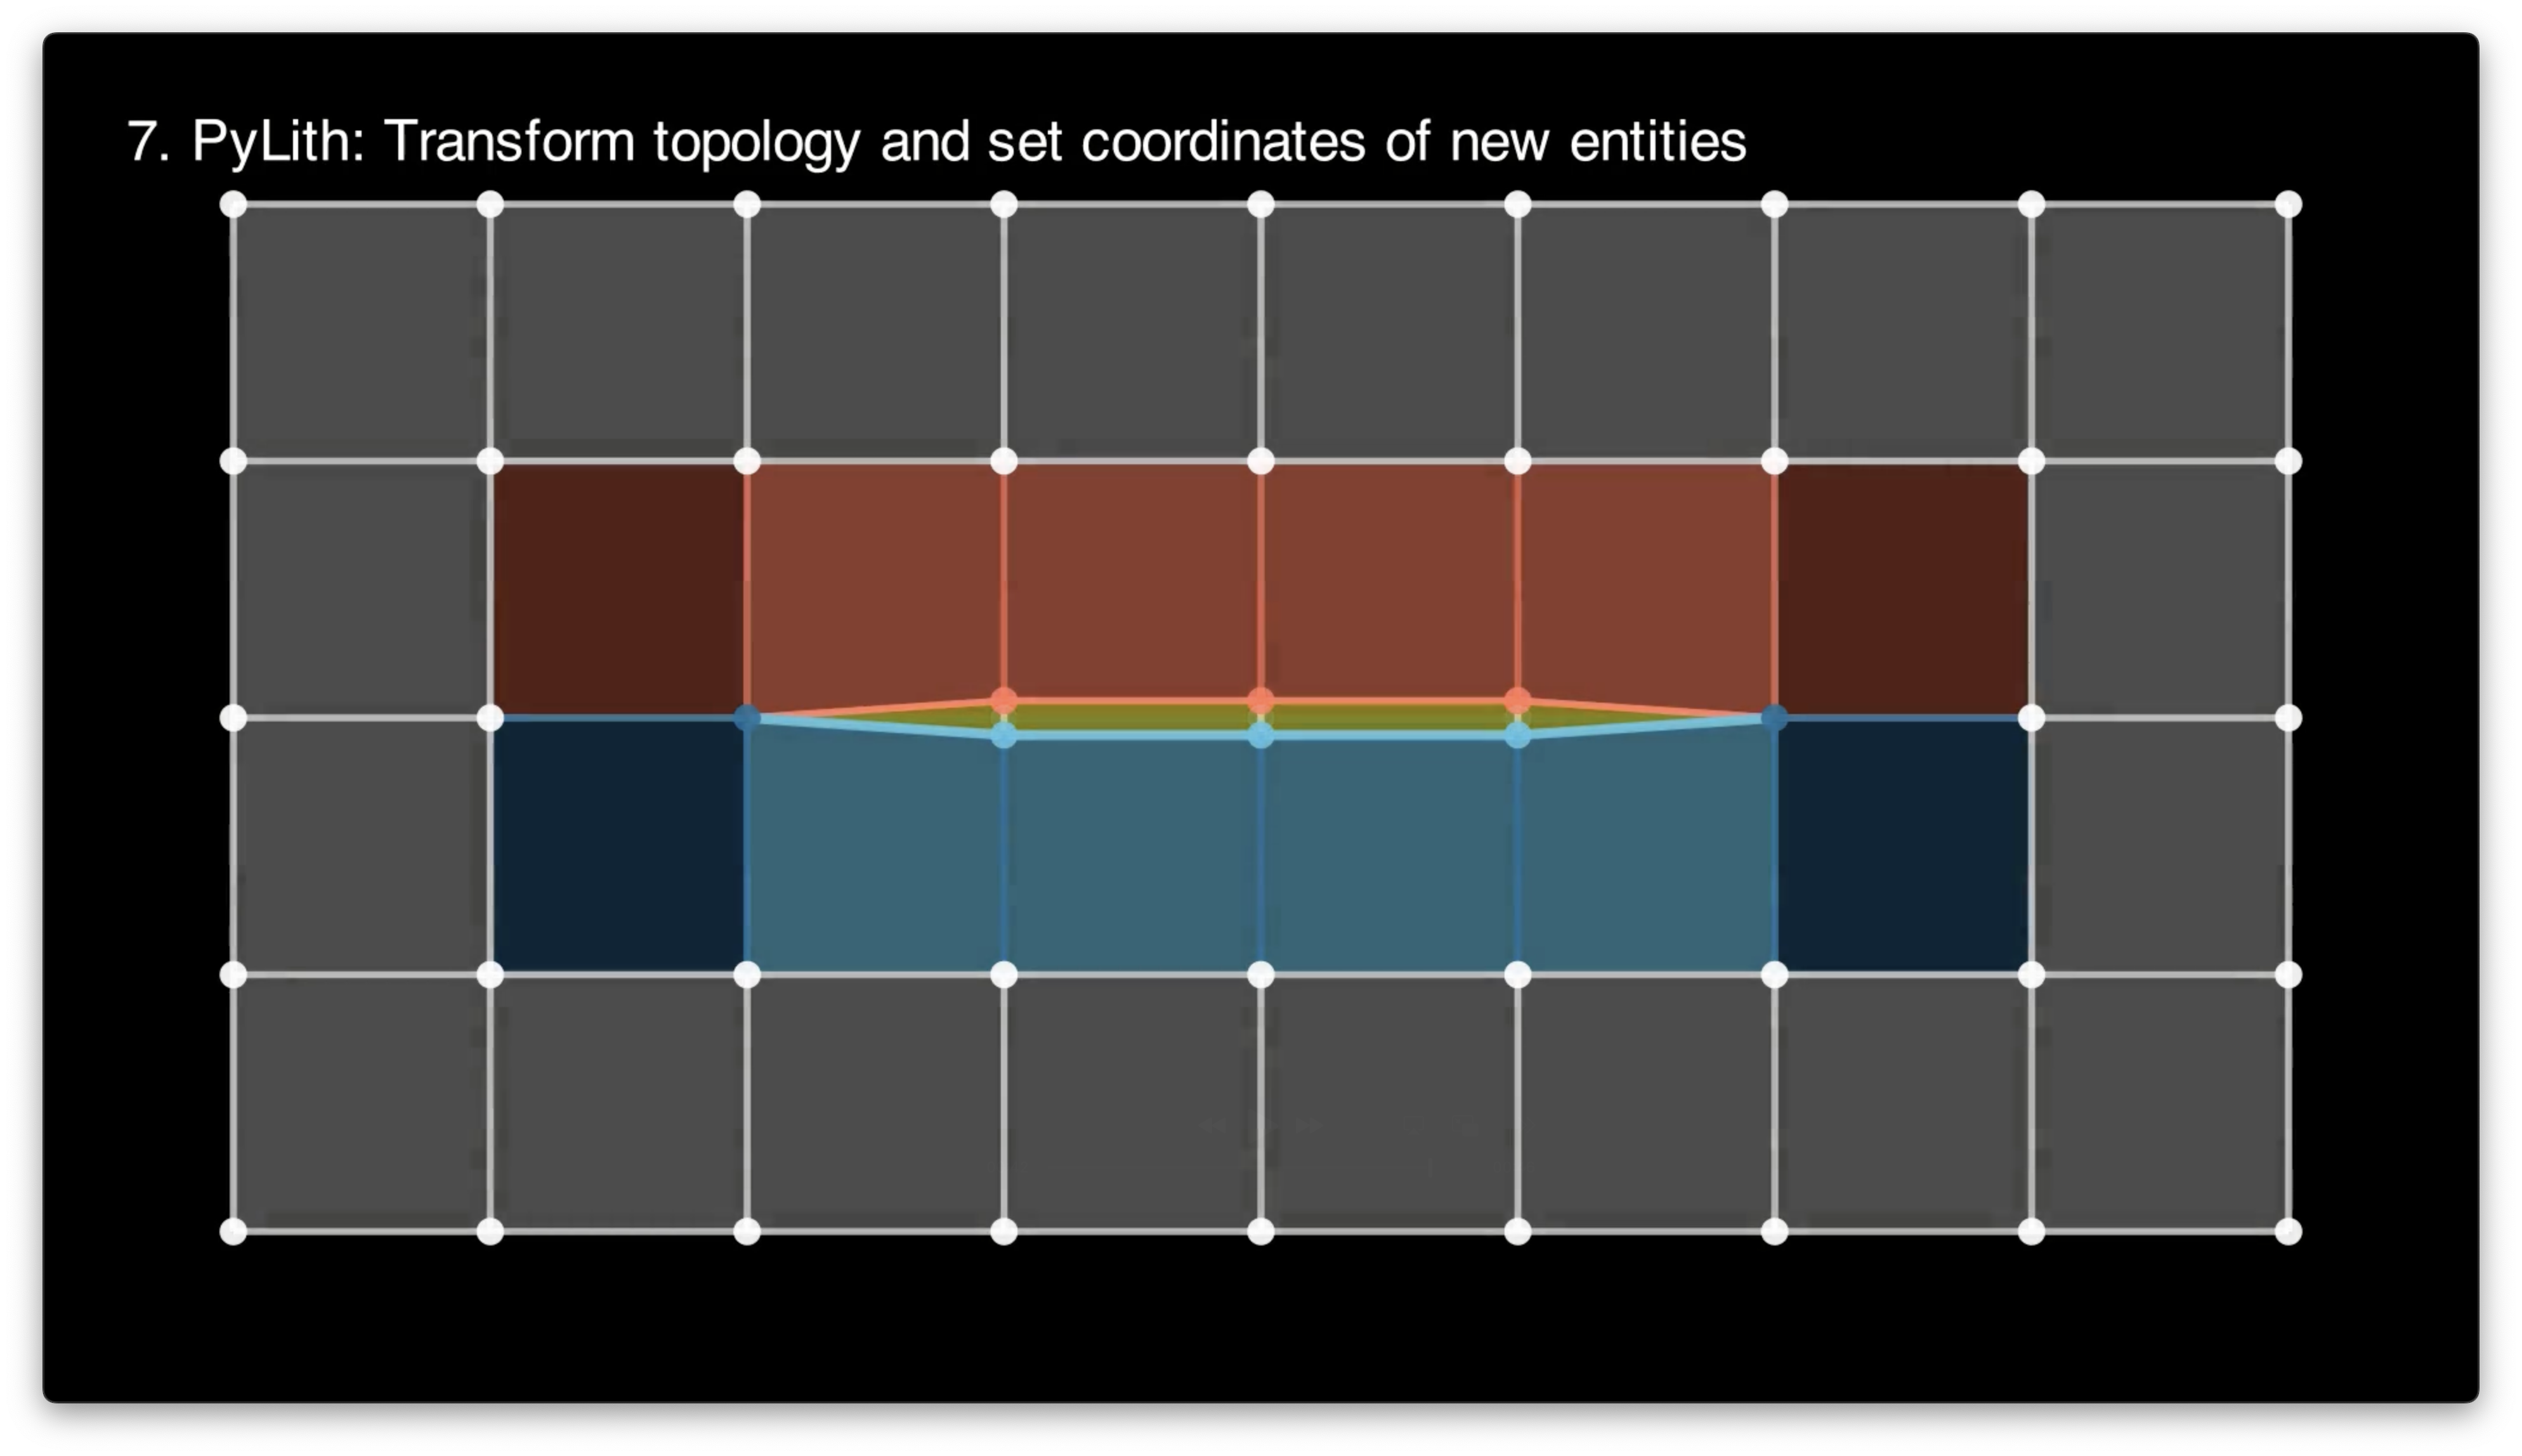
\includegraphics[width=\textwidth]{movies/fault}}
  
\end{frame}


% ------------------------------------------------------------ SLIDE
\begin{frame}
  \frametitle{Implementation of faults with cohesive cells}
  \summary{}

  \begin{itemize}
  \hitem{Advantages}
    \begin{itemize}
    \item Fault formulation is limited to cohesive cells
    \item Bulk material formulation is independent of faults
    \item Mesh generation only needs to mark the faces (edges in 2D) of faults
    \end{itemize}
  \hitem{Disadvantages}
    \begin{itemize}
    \item Domain decomposition with Lagrange multipliers yields a system of equations with a saddle-point
      \begin{equation}
        A s = b \text{, where }
        A =
        \begin{bmatrix}
          \tensor{K} & \tensor{L}^{T} \\
          \tensor{L} & \tensor{0}
        \end{bmatrix}
        \text{ and }
        s = 
        \begin{bmatrix}
          \bm{u} \\
          \bm{l}
        \end{bmatrix}
      \end{equation}
    \end{itemize}
  \end{itemize}
  
\end{frame}


% ========================================================== SECTION
\section{Using PyLith}

% ------------------------------------------------------------ SLIDE
\begin{frame}
  \frametitle{Overview of PyLith Workflow}
  \summary{}

  \includefigure[height=7.0cm]{figs/user-workflow}
\end{frame}


% ------------------------------------------------------------ SLIDE
\begin{frame}
  \frametitle{Finite-Element Mesh}
  \summary{}

  \begin{minipage}{0.40\textwidth}
    \includefigure[width=\textwidth]{figs/mesh-quad}
  \end{minipage}
  \hfill
  \begin{minipage}{0.58\textwidth}
    \includefigure[width=\textwidth]{figs/mesh-tet}
  \end{minipage}
  
\end{frame}

% ------------------------------------------------------------ SLIDE
\begin{frame}
  \frametitle{Code Architecture and Dependencies}
  \summary{}

  \includefigure[width=\textwidth]{figs/pylith-packages}

\end{frame}


% ------------------------------------------------------------ SLIDE
\begin{frame}
  \frametitle{Pyre Framework}
  \summary{}

  \begin{minipage}{0.6\textwidth}
    \begin{itemize}
      \item Component-based architecture for building flexible scientific applications
      \item Capture user-input with defaults and validation
      \item Units management
      \item Integrated C++ and Python logging
      \item Launching MPI jobs
      \end{itemize}
  \end{minipage}
  \hfill
  \begin{minipage}{0.38\textwidth}
    \includefigure[width=\textwidth]{figs/pyre-component}
  \end{minipage}

\end{frame}


% ------------------------------------------------------------ SLIDE
\begin{frame}
  \frametitle{A Pyre application is a hierarchy of components}
  \summary{}

  \includefigure[height=7.2cm]{figs/component-hierarchy}

\end{frame}


% ------------------------------------------------------------ SLIDE
\begin{frame}
  \frametitle{Portable Extensible Toolkit for Scientific Computation (PETSc)}
  \summary{\url{petsc.org}}

  \begin{itemize}
    \item Toolkit for solving partial differential equations (PDEs)
    \item Solvers + preconditioners
    \item Parallel data structures (vectors, matrices)
    \item Finite-element data structures
    \item Mesh input (Gmsh, \ldots) and HDF5 output
  \end{itemize}

\end{frame}

% ------------------------------------------------------------ SLIDE
\begin{frame}
  \frametitle{Meshing Software Compatible with PyLith}
  \summary{}

  \begin{itemize}
    \hitem{Cubit}
    \begin{itemize}
      \item User-friendly GUI
      \item Linux and Windows; MacOS no longer supported
      \item Closed source; free for government use
      \item Scripting with Python or Cubit-specific scripting language
    \end{itemize}
    \hitem{Gmsh}
    \begin{itemize}
      \item Simple GUI
      \item Linux, Windows, and MacOS
      \item Open-source; distributed via PyPI
      \item Scripting with Python or Gmsh-specific scripting language
    \end{itemize}
    \hitem{PyLith-specific ASCII files}
    \begin{itemize}
      \item Simple text files
      \item Good for toy examples and testing
    \end{itemize}
  \end{itemize}

\end{frame}


% ------------------------------------------------------------ SLIDE
\begin{frame}
  \frametitle{Defaults, Modularity, and Extensibility}
  \summary{}

  \begin{itemize}
    \hitem{Defaults target quasi-static elasticity}
    \begin{itemize}
    \item Time-dependent problem
    \item Elasticity governing equation
    \item Linear, isotropic elastic bulk rheology
    \item Dirichlet (displacement) boundary conditions
    \end{itemize}
    \hitem{General defaults}
    \begin{itemize}
    \item SimpleDB spatial database
    \item Write data to HDF5 files
    \end{itemize}
    \hitem{Modular and Extensible}
    \begin{itemize}
    \item Select alternative components at runtime
    \item Additional alternative components can be added without modifying PyLith
    \end{itemize}
  \end{itemize}
  
\end{frame}


% ------------------------------------------------------------ SLIDE
\begin{frame}[fragile]
  \frametitle{Parameter Files}
  \summary{Simple syntax for specifying parameters for properties and components}

  Syntax\vspace*{-4pt}%
  \begin{cfgcode}
    [pylithapp.COMPONENT.SUBCOMPONENT]
    COMPONENT = OBJECT
    PARAMETER = VALUE
  \end{cfgcode}

  \vspace*{-0pt}%
  Example\vspace*{-4pt}%
  \begin{cfgcode}
      [pylithapp.problem]
      bc = [bc_xneg, bc_xpos]
      bc.bc_xneg = pylith.bc.DirichletTimeDependent
      bc.bc_xpos = pylith.bc.DirichletTimeDependent

      [pylithapp.problem.bc.bc_xpos]
      constrained_dof = [0]
      label = boundary_xpos

      db_auxiliary_field = spatialdata.spatialdb.UniformDB
      db_auxiliary_field.description = Dirichlet BC on +x boundary
      db_auxiliary_field.values = [initial_amplitude_x, initial_amplitude_y]
      db_auxiliary_field.data = [+2.0*m, 0*m]
    \end{cfgcode}
  
\end{frame}


% ------------------------------------------------------------ SLIDE
\begin{frame}
  \frametitle{Spatial Databases}
  \summary{User-specified field/value in space for properties and boundary condition values.}

  \begin{itemize}
 \item Examples
    \begin{itemize}
    \item Uniform value for Dirichlet BC (0D)
    \item Piecewise linear variation in tractions for Neumann BC (1D)
    \item Distribution of slip on a fault (2D)
    \item 3D seismic velocity model (3D)
    \end{itemize}\pause
  \item Generally independent of discretization for problem\pause
  \item Available spatial databases
    \begin{description}
    \item[AnalyticDB] Analytical functional form
    \item[UniformDB] Optimized for uniform value
    \item[SimpleDB] Arbitrarily distributed points for variations in 0D, 1D, 2D, or 3D
    \item[SimpleGridDB] Logically gridded points for variations in 1D, 2D, or 3D
    \item[ZeroDB] Special case of UniformDB with zero values
    \end{description}
 \end{itemize}

\end{frame}


% ------------------------------------------------------------ SLIDE
\begin{frame}
  \frametitle{Testing}
  \summary{We have used continuous integration (CI) testing since 2006}

  \begin{itemize}
    \item Continuous integration testing
    \begin{itemize}
      \item Unit tests (small pieces of code, e.g. functions)
      \item Method of Manufactured Solutions (MMS) tests (verify numerical implementation)
      \item Full-scale tests (verify simulations produce correct output)
    \end{itemize}
    \item Benchmarks (compare performance across versions)
    \end{itemize}

\end{frame}



% ------------------------------------------------------------ SLIDE
\begin{frame}
  \frametitle{Documentation}
  \summary{Documentation is online; EPub and PDF files are also available}

  \begin{description}
  \item[PyLith] \url{pylith.readthedocs.io}
  \item[SpatialData] \url{spatialdata.readthedocs.io}
  \item[PyLith Installer] \url{pylith_installer.readthedocs.io}
  \end{description}
  
\end{frame}


% ------------------------------------------------------------ SLIDE
\begin{frame}[t]
  \frametitle{Navigating the PyLith Manual}
  \summary{}

  \begin{itemize}
    \hitem{Introduction}
    \begin{onlyenv}<1>
      \begin{enumerate}
      \item Preface
      \item Conventions
      \item Quickstart
      \item Release Notes
      \item Development Plan
      \end{enumerate}
    \end{onlyenv}
  \hitem{User Guide -- Introduction}
    \begin{onlyenv}<2>
      \begin{enumerate}
      \item Release information
      \item History
      \item PyLith Workflow
      \item Architecture
      \item Getting Help and Reporting Bugs
      \end{enumerate}
    \end{onlyenv}
  \hitem{User Guide -- Running PyLith}
    \begin{onlyenv}<3>
      \begin{enumerate}
      \item Defining the Simulation
      \item PyLith Application
      \item PETSc Options
      \item Finite-Element Mesh
      \item Utilities
      \item Troubleshooting
      \end{enumerate}
    \end{onlyenv}
    \hitem{User Guide -- PyLith Components}
    \begin{onlyenv}<4>
      \begin{itemize}
      \item Full name and journal name
      \item List of Pyre properties and components with default values
      \item Example of setting parameters in a \pylith{cfg} file
      \end{itemize}
    \end{onlyenv}
    \hitem{Developer Guide -- Contributing to PyLith}
    \begin{onlyenv}<5>
      \begin{enumerate}
      \item Coding Style
      \item Git Workflow
      \item Code Layout
      \item PETSc Finite-Element Implementation
      \item Adding New Governing Equations or Bulk Rheologies
      \item Rebuilding PETSc and PyLith
      \item Contributing to Documentation
      \end{enumerate}
    \end{onlyenv}
  \end{itemize}

\end{frame}


% ------------------------------------------------------------ SLIDE
\begin{frame}
  \frametitle{Utilities}
  \summary{\url{https://pylith.readthedocs.io/en/latest/user/run-pylith/utilities.html}}

  \begin{description}
    \item[pylith\_viz] Utility for plotting information in HDF5 files output from PyLith
  \item[pyre\_doc] Display the Pyre properties and facilities available for a given component
  \item[pylith\_cfgsearch] Search and display metadata in .cfg files
  \item[pylith\_runner] Run all PyLith simulations in a given path
  \item[pylith\_dumpparameters] Dump simulation parameters, including default values, to a file for viewing
  \item[pylith\_eqinfo] Compute earthquake rupture metrics (moment magnitude, seismic moment, average slip) from PyLith output
  \item[pylith\_genxdmf] Generate Xdmf files from HDF5 files written by PyLith
  \end{description}  
  
\end{frame}


% ------------------------------------------------------------ SLIDE
\begin{frame}
  \frametitle{Parameters Graphical User-Interface}
  \summary{{\tt cd parametersgui; ./pylith\_paramviewer}}

  \includefigure[height=8.5cm]{figs/paramgui-snapshot}

\end{frame}

% ========================================================== SECTION
\section{Getting Started}
\subsection{Steps}

% ------------------------------------------------------------ SLIDE
\begin{frame}
  \frametitle{Getting Started}
  \summary{}

  \begin{itemize}
  \hitem{Read the User Guide sections of the PyLith Manual} \url{https://pylith.readthedocs.io}
  \hitem{Do not ignore error messages and warnings!}
  \item Use an example or benchmark as a starting point
  \item CIG community forums\\
    \url{https://community.geodynamics.org/c/pylith}
  \item Users tab on PyLith webpage\\
    \url{https://geodynamics.org/resoures/pylith/users}
  \end{itemize}

\end{frame}


% ------------------------------------------------------------ SLIDE
\begin{frame}[t]
  \frametitle{Creating a Simulation}
  \summary{}

  \begin{enumerate}
  \item Create a diagram of the boundary value problem
  \item Generate the finite-element mesh
    \begin{onlyenv}<2>
      \begin{enumerate}
      \item Create a diagram of the geometry
      \item Create the geometry
      \item Mark boundaries (Gmsh)
      \item Generate the mesh
      \item \important{Check mesh quality}
      \end{enumerate}
    \end{onlyenv}
  \item Create the parameter file(s)
    \begin{onlyenv}<3>
      \begin{enumerate}
      \item Select the governing equation (material)
      \item Set solution field based on governing equation
      \item Set solution field basis order based on spatial variation of solution
      \item Choose output (domain, boundary, points) and fields
      \item Set materials and bulk rheologies based on governing equation
      \item Set faults and ruptures
      \item Set boundary conditions
      \item Set basis order of auxiliary subfields based on spatial variation
      \item Set metadata
      \end{enumerate}
    \end{onlyenv}
  \item Create the spatial databases
    \begin{onlyenv}<4>
      \begin{enumerate}
      \item Select the data dimension (point=0, line=1, surface=2, volume=3)
      \item Select spatial database implementation
        \begin{itemize}
        \item \pylith{AnalyticalDB}
        \item \pylith{UniformDB}
        \item \pylith{SimpleDB} Irregular point distribution
        \item \pylith{SimpleGridDB} Points on logical grid aligned with coordinate axes
        \end{itemize}
      \end{enumerate}
    \end{onlyenv}
  \end{enumerate}
  
\end{frame}

% ------------------------------------------------------------ SLIDE
\begin{frame}
  \frametitle{General Tips}
  \summary{}

  \begin{itemize}
    \hitem{Start simple}
    \begin{itemize}
    \item Start in 2D
    \item Simplify the geometry
    \item Use a coarse mesh
    \item Use a static simulation
    \item Use prescribed slip
    \end{itemize}
    \hitem{Increase complexity in steps}
    \begin{enumerate}
    \item Add time dependence
    \item Increase mesh resolution where needed
    \item Transition to spontaneous rupture
    \item Transition to 3D
    \item Increase resolution of geometry
    \end{enumerate}
  \end{itemize}
  
\end{frame}


% ========================================================== SECTION
\subsection{PyLith}

% ------------------------------------------------------------ SLIDE
\begin{frame}[fragile]
  \frametitle{First Steps}
  \summary{}

  \begin{enumerate}
    \hitem{Create a play area for working with examples}
    \begin{bashcode}
      cd PATH_TO_PYLITH_DIR
      mkdir playpen
      cp -r src/pylith-5.0.0/examples playpen/
    \end{bashcode}
  \item Work through relevant examples
  \item Try to complete relevant exercises listed in the manual
  \item Modify an example to look like your problem of interest
  \end{enumerate}

\end{frame}

 
% ======================================================================
\end{document}


% End of file
